% Rapport technique du projet SOA : gestion intelligente des stages et des offres de recrutement.
% Compilation : .\compiler.ps1 (XeLaTeX, deux passes) ou, sur Overleaf, compilateur XeLaTeX.
% Les fichiers de generes/ sont produits par les scripts de outils/ à partir des contrats et des rapports de test.
\documentclass[11pt, a4paper, openany]{report}
% Préambule du rapport : mise en page, polices, couleurs, environnements. Compilation : XeLaTeX (voir compiler.ps1).
\usepackage{fontspec}
\usepackage[french]{babel}
\usepackage{geometry}
\geometry{a4paper, top=24mm, bottom=24mm, left=25mm, right=22mm, headheight=14pt}

% Polices : Latin Modern, la police standard de LaTeX (même rendu que les rapports de TP du module).
\setmainfont{Latin Modern Roman}[SmallCapsFont={Latin Modern Roman Caps}]
\setsansfont{Latin Modern Sans}
\setmonofont{Latin Modern Mono}[Scale=1.02, BoldFont={lmmonolt10-bold.otf}]
\newcommand{\titres}{\rmfamily}

\usepackage{xcolor}
\definecolor{inpt}{HTML}{0B5A99}   % bleu des titres : bleu du logo INPT (007BC7) assombri pour la lecture
\definecolor{inptpale}{HTML}{EAF3FA}
\definecolor{encre}{HTML}{000000}
\definecolor{encre2}{HTML}{4A4A4A}
\definecolor{filet}{HTML}{000000}
\definecolor{papier}{HTML}{F5F7FA}
\definecolor{ok}{HTML}{1F6B3A}
\definecolor{ko}{HTML}{9B2C2C}
\definecolor{attente}{HTML}{8A5A00}
\color{encre}

\usepackage{microtype}
\usepackage{graphicx}
\graphicspath{{figures/}}
\usepackage{float}
\usepackage{booktabs}
\usepackage{longtable}
\usepackage{tabularx}
\usepackage{array}
\usepackage{rotating}
\usepackage{setspace}
\setstretch{1.08}
\usepackage{ragged2e}
\usepackage{amsmath}
\usepackage{etoolbox}
\usepackage{afterpage}

\usepackage{tikz}
\usetikzlibrary{positioning, arrows.meta, shapes.geometric, shapes.misc, shapes.multipart, fit, calc, backgrounds}
\usepackage{tcolorbox}
\usepackage{listings}

% Titres
\usepackage{titlesec}
\titleformat{\chapter}[hang]
  {\huge\bfseries\color{inpt}}
  {\thechapter.}
  {0.5em}
  {}
\titlespacing*{\chapter}{0pt}{-12pt}{16pt}
\titleformat{\section}{\Large\bfseries\color{inpt}}{\thesection}{0.8em}{}
\titleformat{\subsection}{\large\bfseries\color{inpt}}{\thesubsection}{0.8em}{}
\titleformat{\subsubsection}{\normalsize\bfseries\color{encre}}{}{0em}{}
\titlespacing*{\section}{0pt}{18pt}{8pt}
\titlespacing*{\subsection}{0pt}{14pt}{6pt}

% En-têtes et pieds de page
\usepackage{fancyhdr}
\pagestyle{fancy}
\fancyhf{}
\renewcommand{\headrulewidth}{0.4pt}
\renewcommand{\headrule}{{\color{filet}\hrule height\headrulewidth width\headwidth}}
\fancyhead[L]{\small\color{inpt}Projet SOA -- Gestion des stages}
\fancyhead[R]{\small\color{inpt}INPT -- \textsc{Module SOA}}
\fancyfoot[C]{\small\thepage}
\renewcommand{\chaptermark}[1]{\markboth{#1}{}}
\fancypagestyle{plain}{\fancyhf{}\renewcommand{\headrulewidth}{0pt}\renewcommand{\headrule}{}\fancyfoot[C]{\small\thepage}}

% Légendes (sans le paquet caption, absent de l'installation MiKTeX de base)
\makeatletter
\renewcommand{\fnum@figure}{\textsc{Figure}~\thefigure}
\renewcommand{\fnum@table}{\textsc{Tableau}~\thetable}
% « Figure 1 – texte », comme dans les rapports de TP
\long\def\@makecaption#1#2{\vskip\abovecaptionskip
  \sbox\@tempboxa{#1 -- #2}%
  \ifdim \wd\@tempboxa >\hsize #1 -- #2\par\else\global\@minipagefalse\hb@xt@\hsize{\hfil\box\@tempboxa\hfil}\fi
  \vskip\belowcaptionskip}
\makeatother

\usepackage[hidelinks, pdfusetitle]{hyperref}
\hypersetup{pdfauthor={Hiba Elamdaoui, Aya Zahri, Hibatollah Ait Ahmed}, pdftitle={Gestion intelligente des stages et des offres de recrutement}}
\urlstyle{tt}

% Code
\lstdefinestyle{code}{
  basicstyle=\ttfamily\footnotesize,
  columns=fullflexible, keepspaces=true,
  breaklines=true, breakatwhitespace=false, postbreak=\mbox{\textcolor{filet}{$\hookrightarrow$}\space},
  frame=leftline, framerule=1.6pt, rulecolor=\color{inpt}, framesep=8pt, xleftmargin=10pt,
  backgroundcolor=\color{papier},
  aboveskip=10pt, belowskip=10pt,
  showstringspaces=false, tabsize=2,
  commentstyle=\color{encre2}\itshape, stringstyle=\color{inpt}, keywordstyle=\color{encre}\bfseries,
}
\lstdefinelanguage{XMLfr}{morestring=[b]", morecomment=[s]{<!--}{-->}, alsoletter={:-}, sensitive=true}
\lstdefinelanguage{JSONfr}{morestring=[b]", sensitive=true}
\lstdefinelanguage{HTTPfr}{morestring=[b]", sensitive=true, morecomment=[l]{-->}}
\lstset{style=code}

% Encadrés
% (bibliothèques « skins » de tcolorbox non utilisées : elles exigent tikzfill, absent de MiKTeX de base)
\newenvironment{encadre}[1][]
  {\begin{tcolorbox}[colback=inptpale, colframe=inpt, boxrule=0pt, leftrule=2pt, arc=0pt, left=10pt, right=10pt, top=6pt, bottom=6pt]%
   \ifstrempty{#1}{}{{\titres\bfseries\small\color{inpt}#1}\par\smallskip}}
  {\end{tcolorbox}}

% Emplacement de capture d'écran : affiché tant que le fichier n'est pas dans figures/.
\newcommand{\emplacement}[2]{%
  \begin{tikzpicture}
    \node[draw=encre2, dashed, line width=0.8pt, fill=papier, minimum width=\linewidth-1pt, minimum height=#2, align=center, text width=0.8\linewidth]
      {{\titres\bfseries\color{ko}CAPTURE À FAIRE}\\[4pt]
       {\small\texttt{rapport/figures/\detokenize{#1}}}\\[2pt]
       {\footnotesize\color{encre2}Voir \texttt{docs/CAPTURES\_A\_FAIRE.md}}};
  \end{tikzpicture}}

% \capture{fichier}{hauteur de l'emplacement}{légende}{étiquette} : capture faite à la main (Bonita, SoapUI, Postman).
\newcommand{\capture}[4]{%
  \begin{figure}[htbp]\centering
    % L'emplacement vide reste compact (34 mm) ; la capture réelle prend la place nécessaire.
    \IfFileExists{figures/#1}{\includegraphics[width=\linewidth,height=0.45\textheight,keepaspectratio]{#1}}{\emplacement{#1}{34mm}}
    \caption{#3}\label{#4}
  \end{figure}}

% \ecran{fichier}{hauteur gardée en px}{hauteur totale en px}{largeur}{légende}{étiquette} : capture de l'interface (Playwright),
% coupée en haut de page quand elle est très haute.
\newcommand{\ecran}[6]{%
  \begin{figure}[H]\centering
    {\setlength{\fboxsep}{0pt}\color{filet}\fbox{\includegraphics[width=#4\linewidth, viewport=0 {\numexpr #3-#2\relax} 1360 #3, clip]{#1}}}
    \caption{#5}\label{#6}
  \end{figure}}

% Divers
% Lignes de tableau générées : \input n'est pas développable dans un tableau, la primitive \@@input l'est.
\makeatletter\newcommand{\lignes}[1]{\@@input #1 }\makeatother
\newcommand{\code}[1]{\texttt{#1}}
\newcommand{\regle}[1]{\textbf{\textcolor{inpt}{#1}}}
\newcommand{\statut}[1]{\textsf{\small #1}}
\setlength{\parskip}{4pt plus 1pt}
\setlength{\parindent}{0pt}
\setlength{\emergencystretch}{3em}  % évite les débordements dus aux termes en chasse fixe
\renewcommand{\arraystretch}{1.25}
\setlength{\LTpre}{8pt}
\setlength{\LTpost}{8pt}
% Listes plus serrées (sans enumitem)
\makeatletter
\def\@listi{\leftmargin\leftmargini \topsep 4pt \parsep 1pt \itemsep 2pt}
\let\@listI\@listi
\makeatother

% Généré par rapport/outils/resultats_tests.py à partir des rapports de test. Ne pas modifier.
\newcommand{\nbJunit}{356}
\newcommand{\nbJunitIT}{44}
\newcommand{\nbSoapUI}{546}
\newcommand{\nbPostmanRequetes}{87}
\newcommand{\nbPostman}{226}
\newcommand{\nbBoutEnBout}{65}
\newcommand{\modeBoutEnBout}{bonita}


\begin{document}

\pagenumbering{roman}
% Page de couverture, sur le modèle des rapports de TP du module (logos ANRT et INPT, bâtiment de l'INPT en pied de page).
\begin{titlepage}
\thispagestyle{empty}
\newgeometry{top=18mm, bottom=18mm, left=22mm, right=22mm}
\centering

\begin{minipage}[c]{0.5\textwidth}\raggedright
  
\includegraphics[height=21mm]{logo-anrt.png}
\end{minipage}%
\begin{minipage}[c]{0.5\textwidth}\raggedleft
  
\includegraphics[height=19mm]{logo-inpt.png}
\end{minipage}

\vspace{26mm}
{\Large\textsc{Filière Innovation \& AMOA}\par}
\vspace{6mm}
{\LARGE RAPPORT DE PROJET\par}
\vspace{9mm}
{\color{encre}\rule{0.72\textwidth}{0.9pt}\par}
\vspace{6mm}
{\color{inpt}\huge\bfseries Gestion intelligente des stages\\[3pt] et des offres de recrutement\par}
\vspace{4mm}
{\color{encre}\rule{0.72\textwidth}{0.9pt}\par}

\vspace{14mm}
{\large\textbf{Thème :} architecture orientée services, trois services SOAP, trois services REST\\[2pt]
et un processus BPMN orchestré par Bonita.\par}

\vspace{24mm}
\begin{minipage}[t]{0.48\textwidth}\raggedright\large
  \textbf{Réalisé par :}\\[4pt]
  Hiba \textsc{Elamdaoui}\\
  Aya \textsc{Zahri}\\
  Hibatollah \textsc{Ait Ahmed}
\end{minipage}%
\begin{minipage}[t]{0.48\textwidth}\raggedleft\large
  \textbf{Enseignant :}\\[4pt]
  Pr. Hatim \textsc{Guermah}
\end{minipage}

\vspace{12mm}
{\large\textbf{Module :} SOA\par}

\vfill

\includegraphics[height=17mm]{logo-zlafa.png}\par
\vspace{5mm}
{\large\textsc{Agence Nationale de Réglementation des Télécommunications}\\[2pt]
\textsc{Institut National des Postes et Télécommunications}\par}
\vspace{2mm}
{Année universitaire : 2026/2027\par}

\restoregeometry
\end{titlepage}

% Remerciements et résumé
\chapter*{Remerciements}
\addcontentsline{toc}{chapter}{Remerciements}
\markboth{Remerciements}{}

Nous remercions Pr.~Hatim \textsc{Guermah}, qui a encadré ce projet dans le cadre du module SOA, pour un sujet qui nous a fait traverser toute la chaîne d'une architecture orientée services : contrats, sécurité des échanges, orchestration et tests.

Nos remerciements vont aussi à l'équipe pédagogique de la filière AMOA de l'INPT, dont les enseignements de modélisation des processus et d'analyse des besoins ont directement servi à la conception du processus de candidature.

Enfin, merci aux communautés qui maintiennent les outils libres utilisés ici : Eclipse Metro (JAX-WS), Eclipse Jersey (JAX-RS), MySQL, Mailpit, Bonita Community, SoapUI Open Source, Newman et bpmn-js.

\chapter*{Résumé}
\addcontentsline{toc}{chapter}{Résumé}
\markboth{Résumé}{}

Ce rapport présente une plateforme de gestion des stages réalisée selon une architecture orientée services. Six services indépendants, chacun avec sa propre base de données, couvrent les étudiants, les entreprises partenaires et les offres de stage (services SOAP décrits par des contrats WSDL), ainsi que les candidatures, les notifications et le suivi des stages (services REST décrits par des contrats OpenAPI).

Le traitement d'une candidature, du dépôt à la décision de l'entreprise puis à la création du dossier de stage, est modélisé par un processus BPMN exécuté dans Bonita, qui appelle les six services. Onze règles de gestion, numérotées de R1 à R11, encadrent ce traitement : éligibilité de l'étudiant, validité de l'offre, date limite, places, doublons, nombre de candidatures actives, compatibilité du profil, annulation, transitions de statut, acceptation et demande de complément.

Les échanges SOAP sont authentifiés par WS-Security, les appels REST par une clé d'API par client, et les utilisateurs par un portail avec trois rôles. Les pannes de service sont traitées par le processus comme par le portail, et un identifiant de corrélation permet de suivre une candidature dans les journaux de tous les services.

Le projet est vérifié par \nbJunit{} tests JUnit (dont \nbJunitIT{} sur la vraie base de données), \nbSoapUI{} assertions SoapUI, \nbPostman{} assertions Postman et un test de bout en bout qui rejoue chaque scénario par le portail et contrôle les courriels reçus. Une interface web, proposée en bonus, permet aux étudiants de candidater, aux entreprises de décider et au responsable de suivre les stages, avec l'avancement de chaque candidature affiché sur le diagramme BPMN.

\bigskip
\textbf{Mots-clés :} architecture orientée services, SOAP, WSDL, JAX-WS, REST, JAX-RS, OpenAPI, BPMN, Bonita, orchestration, WS-Security, MySQL.


\tableofcontents
\listoffigures
\listoftables

\cleardoublepage
\pagenumbering{arabic}
\chapter{Introduction et contexte}\label{chap:introduction}

\section{Contexte}

Les établissements d'enseignement supérieur gèrent chaque année des centaines d'offres de stage et des milliers de candidatures. À l'INPT, comme dans beaucoup d'écoles, ces échanges passent encore largement par des courriels et des tableurs : l'entreprise publie une offre, les étudiants envoient leur dossier, le service des stages vérifie à la main l'éligibilité de chacun, relance les entreprises et reporte les décisions. Les informations sont dispersées, les règles appliquées de façon inégale et le suivi d'un dossier repose sur la mémoire des personnes.

Le sujet du projet propose de remplacer ce fonctionnement par une plateforme fondée sur une \textbf{architecture orientée services} (SOA). Chaque domaine du métier (étudiants, entreprises, offres, candidatures, notifications, suivi des stages) devient un service autonome, qui expose un contrat et garde ses propres données. Un \textbf{processus BPMN} orchestre ces services pour traiter une candidature de bout en bout, du dépôt jusqu'à la décision finale.

\section{Objectifs}

Le cahier des charges fixe les livrables suivants :
\begin{itemize}
  \item trois services \textbf{SOAP} décrits par WSDL : gestion des étudiants (S1), des entreprises (S2) et des offres de stage (S3) ;
  \item trois services \textbf{REST} : gestion des candidatures (S4), notifications (S5) et suivi des stages (S6) ;
  \item un \textbf{processus BPMN} modélisé et exécuté dans Bonita Studio, qui orchestre les appels SOAP et REST, gère les décisions, les erreurs et les notifications ;
  \item un \textbf{rapport technique} et une \textbf{vidéo de démonstration} ;
  \item en bonus, une \textbf{interface graphique} pour les étudiants, les entreprises et le responsable des stages.
\end{itemize}

Nous avons ajouté trois exigences de qualité, qui guident les choix décrits dans la suite : chaque service doit pouvoir être testé seul, chaque règle de gestion doit être vérifiée par un test automatique, et aucune panne d'un service ne doit laisser une candidature dans un état incohérent.

\section{Choix techniques}

Nous avons suivi les technologies recommandées par l'énoncé :

\begin{table}[H]
\centering\small
\begin{tabularx}{\linewidth}{@{}l>{\raggedright\arraybackslash}X@{}}
\toprule
\textbf{Domaine} & \textbf{Choix} \\ \midrule
Langage & Java 17, projet Maven multi-module (un module par service, plus un socle commun) \\
SOAP & JAX-WS (Eclipse Metro 4), WSDL écrits d'abord (\emph{contract first}), clients générés par \code{wsimport} \\
REST & JAX-RS (Eclipse Jersey 3.1) sur un serveur Grizzly, contrats OpenAPI 3 écrits à la main \\
Persistance & MySQL 8.4 dans Docker, un schéma et un compte par service, JDBC avec le pool HikariCP \\
Orchestration & Bonita Studio Community 2025.2 ; mode de secours « direct » exécuté en Java \\
Courriels & SMTP vers Mailpit, serveur de courriel de test (aucun envoi réel) \\
Tests & JUnit 5.11, SoapUI 5.10, Postman et Newman, test de bout en bout en Node.js, Playwright pour l'interface \\
Interface & HTML, CSS et JavaScript sans framework ; bpmn-js pour l'affichage du processus \\
\bottomrule
\end{tabularx}
\caption{Technologies retenues}\label{tab:technologies}
\end{table}

Chaque service est un programme indépendant, lancé dans son propre processus Java et à l'écoute sur son propre port. Aucun service ne lit la base d'un autre : toute information extérieure passe par un appel de service. C'est ce qui rend l'architecture réellement orientée services, et non un monolithe découpé en paquets.

\section{Organisation du rapport}

Le chapitre~\ref{chap:besoins} analyse les besoins et les acteurs. Le chapitre~\ref{chap:architecture} décrit l'architecture et les interactions entre services, avec le parcours complet d'une candidature. Les chapitres~\ref{chap:soap} et~\ref{chap:rest} documentent les opérations SOAP et les API REST. Le chapitre~\ref{chap:regles} détaille les règles de gestion R1 à R11, et le chapitre~\ref{chap:bpmn} le processus BPMN. Le chapitre~\ref{chap:securite} traite de la sécurité et de la gestion des erreurs, le chapitre~\ref{chap:tests} des scénarios et des résultats de test. Les chapitres~\ref{chap:interface} et~\ref{chap:deploiement} présentent l'interface et le déploiement. Le dernier chapitre discute les limites et les améliorations possibles.

\begin{encadre}[Données de démonstration]
Toutes les personnes, entreprises, adresses et numéros cités dans ce rapport sont fictifs. Les courriels ne quittent jamais la machine : ils sont reçus par Mailpit.
\end{encadre}

\chapter{Analyse des besoins}\label{chap:besoins}

\section{Acteurs}

L'analyse du sujet fait apparaître trois acteurs humains et deux acteurs techniques.

\begin{table}[H]
\centering\small
\begin{tabularx}{\linewidth}{@{}l>{\raggedright\arraybackslash}X@{}}
\toprule
\textbf{Acteur} & \textbf{Rôle} \\ \midrule
Étudiant & Consulte les offres ouvertes, vérifie sa compatibilité avec chacune, candidate, suit ses candidatures, peut annuler tant que l'évaluation n'a pas commencé, consulte son stage. \\
Entreprise partenaire & Publie et gère ses offres, reçoit les candidatures, ouvre l'évaluation, accepte, refuse ou demande un complément d'information. \\
Responsable des stages & Gère les référentiels (étudiants, entreprises), consulte toutes les candidatures, suit les stages (statut, comptes rendus, évaluations), surveille les notifications et l'état des services. \\
Processus BPMN (Bonita) & Acteur technique : orchestre le traitement d'une candidature en appelant les six services. \\
Planificateur & Acteur technique : déclenche chaque jour à 8~h les rappels de date limite. \\
\bottomrule
\end{tabularx}
\caption{Acteurs du système}\label{tab:acteurs}
\end{table}

\section{Besoins fonctionnels}

\subsection{Gestion des référentiels}
\begin{itemize}
  \item Créer, consulter, modifier et supprimer un étudiant (matricule, nom, prénom, filière, niveau, coordonnées, compétences) ; changer son statut (\statut{ACTIF}, \statut{SUSPENDU}, \statut{EN\_STAGE}, \statut{DIPLOME}) selon des transitions autorisées ; vérifier son existence et son éligibilité.
  \item Créer, consulter, modifier et supprimer une entreprise (raison sociale, ICE, secteur, adresse, responsable de contact) ; consulter ses offres.
  \item Créer, modifier, clôturer et supprimer une offre (titre, description, compétences requises, filières acceptées, niveau minimum, durée, date limite, nombre de places) ; vérifier sa disponibilité et sa compatibilité avec un étudiant.
\end{itemize}

\subsection{Candidatures}
\begin{itemize}
  \item Déposer une candidature avec une lettre de motivation ; obtenir immédiatement le résultat du contrôle (enregistrée, ou rejetée avec la règle et le motif).
  \item Consulter ses candidatures, leur historique (date, auteur, commentaire de chaque changement) et les étapes du processus.
  \item Annuler une candidature lorsque les règles le permettent.
  \item Pour l'entreprise : ouvrir l'évaluation, puis accepter, refuser ou demander un complément.
\end{itemize}

\subsection{Notifications}
\begin{itemize}
  \item Confirmer le dépôt à l'étudiant ; informer l'entreprise d'une nouvelle candidature.
  \item Notifier l'étudiant d'un rejet (avec le motif), d'une acceptation, d'un refus ou d'une demande de complément.
  \item Envoyer des rappels aux étudiants compatibles qui n'ont pas encore candidaté à une offre dont la date limite approche.
\end{itemize}

\subsection{Suivi des stages}
\begin{itemize}
  \item Créer le dossier de stage d'une candidature acceptée ; consulter son statut et ses dates.
  \item Enregistrer les comptes rendus périodiques et les évaluations (note sur 20 et commentaire).
  \item Consulter l'historique des stages d'un étudiant.
\end{itemize}

\section{Besoins non fonctionnels}

\begin{table}[H]
\centering\small
\begin{tabularx}{\linewidth}{@{}l>{\raggedright\arraybackslash}X@{}}
\toprule
\textbf{Exigence} & \textbf{Réponse apportée} \\ \midrule
Autonomie des services & Un processus, un port et un schéma de base par service ; aucun accès direct aux données d'un autre service. \\
Contrats explicites & WSDL pour S1 à S3, OpenAPI pour S4 à S6, versionnés dans le dépôt ; le code est vérifié contre ces contrats par des tests. \\
Sécurité & WS-Security UsernameToken (SOAP), clé d'API par client (REST), sessions et rôles au portail, mots de passe hachés (BCrypt), masquage des coordonnées. \\
Robustesse & Délais d'attente sur tous les appels, réponse 503 explicite, sous-processus d'erreur BPMN, alerte au responsable. \\
Traçabilité & Historique de chaque changement de statut ; identifiant de corrélation propagé dans tous les appels. \\
Langue & Messages, erreurs, courriels et interface en français. \\
\bottomrule
\end{tabularx}
\caption{Besoins non fonctionnels}\label{tab:non-fonctionnels}
\end{table}

\section{Cas d'utilisation}

La figure~\ref{fig:cas-utilisation} regroupe les principaux cas d'utilisation. Le dépôt d'une candidature \emph{inclut} son traitement par le processus, qui lui-même inclut les vérifications et l'envoi des notifications.

\begin{figure}[H]
\centering
\begin{tikzpicture}[
  font=\sffamily\scriptsize,
  cas/.style={ellipse, draw=inpt, fill=inptpale, line width=0.6pt, minimum width=36mm, minimum height=7.5mm, inner sep=1pt, align=center, text width=31mm},
  acteur/.style={align=center, font=\sffamily\scriptsize},
  lien/.style={draw=encre2, line width=0.45pt},
  inclut/.style={draw=encre2, dashed, -{Stealth[length=2mm]}, line width=0.45pt},
]
\newcommand{\bonhomme}[2]{%
  \begin{scope}[shift={(#1)}]
    \draw[encre, line width=0.7pt] (0,0.42) circle (0.13);
    \draw[encre, line width=0.7pt] (0,0.29) -- (0,-0.05) (-0.2,0.18) -- (0.2,0.18) (0,-0.05) -- (-0.15,-0.3) (0,-0.05) -- (0.15,-0.3);
    \node[acteur, below] at (0,-0.32) {#2};
  \end{scope}}

% Système
\draw[filet, line width=0.8pt] (-4.2,-8.15) rectangle (4.2,5.15);
\node[font=\titres\small\bfseries, anchor=north west, text=encre2] at (-4.1,5.1) {Plateforme des stages};

% Cas étudiant
\node[cas] (offres) at (-2.05,4.2) {Consulter les offres et la compatibilité};
\node[cas] (deposer) at (-2.05,3.1) {Déposer une candidature};
\node[cas] (suivre) at (-2.05,2.0) {Suivre ses candidatures (historique, processus)};
\node[cas] (annuler) at (-2.05,0.9) {Annuler une candidature};
\node[cas] (stage) at (-2.05,-0.2) {Consulter son stage et ses courriels};

% Cas entreprise
\node[cas] (publier) at (2.05,4.2) {Publier et gérer ses offres};
\node[cas] (recevoir) at (2.05,3.1) {Consulter les candidatures reçues};
\node[cas] (evaluer) at (2.05,2.0) {Ouvrir l'évaluation};
\node[cas] (decider) at (2.05,0.9) {Décider : accepter, refuser, demander un complément};

% Processus
\node[cas, fill=white] (traiter) at (0,-1.5) {Traiter la candidature (processus BPMN)};
\node[cas, fill=white] (verifier) at (-2.05,-2.75) {Vérifier étudiant, offre, entreprise (R1 à R7)};
\node[cas, fill=white] (notifier) at (2.05,-2.75) {Notifier par courriel};
\node[cas, fill=white] (creerstage) at (2.05,-1.5) {Créer le dossier de stage (R10)};

% Cas responsable
\node[cas] (referentiels) at (-2.05,-4.15) {Gérer étudiants et entreprises};
\node[cas] (toutes) at (2.05,-4.15) {Consulter toutes les candidatures};
\node[cas] (suivistage) at (-2.05,-5.3) {Suivre les stages (comptes rendus, évaluations)};
\node[cas] (rappels) at (2.05,-5.3) {Envoyer les rappels de date limite};
\node[cas] (supervision) at (0,-6.5) {Superviser les notifications et l'état des services};
\node[cas, fill=white] (connexion) at (0,-7.55) {S'authentifier};

% Acteurs
\bonhomme{-6.0,2.2}{Étudiant}
\bonhomme{6.0,2.6}{Entreprise}
\bonhomme{-6.0,-5.0}{Responsable\\des stages}
\node[draw=encre2, font=\sffamily\scriptsize, align=center, inner sep=3pt] (bonita) at (6.0,-1.6) {«\,système\,»\\Processus\\Bonita};
\node[draw=encre2, font=\sffamily\scriptsize, align=center, inner sep=3pt] (planif) at (6.0,-5.3) {«\,système\,»\\Planificateur};

\coordinate (E) at (-5.75,2.3); \coordinate (P) at (5.75,2.7); \coordinate (R) at (-5.75,-4.9);
\foreach \c in {offres, deposer, suivre, annuler, stage} \draw[lien] (E) -- (\c.west);
\foreach \c in {publier, recevoir, evaluer, decider} \draw[lien] (P) -- (\c.east);
\foreach \c in {referentiels, suivistage, toutes, rappels, supervision} \draw[lien] (R) -- (\c);
\draw[lien] (bonita) -- (traiter.east);
\draw[lien] (planif) -- (rappels.east);

\draw[inclut] (deposer.south) .. controls (-0.8,1.2) and (-0.4,-0.6) .. node[pos=0.55, fill=white, inner sep=1pt, font=\sffamily\tiny] {«\,inclut\,»} (traiter.north);
\draw[inclut] (decider.south) .. controls (1.2,-0.2) .. (traiter.north east);
\draw[inclut] (traiter) -- (verifier);
\draw[inclut] (traiter) -- (notifier);
\draw[inclut] (traiter) -- (creerstage);
\end{tikzpicture}
\caption{Diagramme des cas d'utilisation}\label{fig:cas-utilisation}
\end{figure}

\section{Statuts manipulés}

Quatre cycles de vie structurent le métier. Leurs transitions sont contrôlées par les services eux-mêmes : une transition non prévue est refusée avec une erreur de conflit (faute \code{ConflitFault} en SOAP, code HTTP 409 en REST).

\begin{table}[H]
\centering\small
\begin{tabularx}{\linewidth}{@{}l>{\raggedright\arraybackslash}X@{}}
\toprule
\textbf{Objet} & \textbf{Statuts et transitions autorisées} \\ \midrule
Étudiant (S1) & \statut{ACTIF} $\rightarrow$ \statut{SUSPENDU}, \statut{EN\_STAGE}, \statut{DIPLOME} ; \statut{SUSPENDU} $\rightarrow$ \statut{ACTIF} ; \statut{EN\_STAGE} $\rightarrow$ \statut{ACTIF}, \statut{DIPLOME} \\
Offre (S3) & \statut{BROUILLON}, \statut{ACTIVE}, \statut{POURVUE} (plus aucune place), \statut{CLOTUREE} \\
Candidature (S4) & \statut{DEPOSEE} $\rightarrow$ \statut{EN\_COURS\_EVALUATION} $\rightarrow$ \statut{ACCEPTEE} ou \statut{REFUSEE} ; \statut{DEPOSEE} $\rightarrow$ \statut{ANNULEE} (règle R9) \\
Stage (S6) & \statut{PLANIFIE} $\rightarrow$ \statut{EN\_COURS} ou \statut{INTERROMPU} ; \statut{EN\_COURS} $\rightarrow$ \statut{TERMINE} ou \statut{INTERROMPU} \\
\bottomrule
\end{tabularx}
\caption{Cycles de vie des principaux objets}\label{tab:statuts}
\end{table}

Une \textbf{soumission} (S4) précède la candidature : c'est la demande de l'étudiant telle qu'elle entre dans le processus. Elle devient \statut{ENREGISTREE} (une candidature est alors créée), \statut{REJETEE} (avec la règle violée et le motif) ou \statut{ERREUR} (un service n'a pas répondu). Cette distinction garde une trace des dépôts refusés sans les compter comme des candidatures.

\chapter{Architecture orientée services}\label{chap:architecture}

\section{Vue d'ensemble}

La plateforme est composée de six services métier, d'un orchestrateur et d'un portail (figure~\ref{fig:architecture}). Chaque service est un processus Java distinct, démarré seul, avec son port et son schéma de base de données. Les services de référentiel (S1 à S3) exposent des opérations SOAP ; les services de traitement (S4 à S6) exposent des ressources REST.

\begin{figure}[H]
\centering
\begin{tikzpicture}[
  font=\sffamily\scriptsize,
  svc/.style={draw=inpt, fill=inptpale, line width=0.7pt, minimum width=30mm, minimum height=14mm, align=center},
  ext/.style={draw=encre2, fill=white, line width=0.6pt, minimum width=30mm, minimum height=11mm, align=center},
  couche/.style={draw=filet, line width=0.8pt, rounded corners=1pt, inner sep=3.5mm},
  appel/.style={-{Stealth[length=2.2mm]}, line width=0.65pt},
  etiq/.style={font=\sffamily\tiny, fill=white, inner sep=1.5pt},
]
% Clients et orchestration
\node[ext] (nav) at (-3.6,8.6) {\textbf{Navigateur}\\étudiant, entreprise, responsable};
\node[svc] (portail) at (-3.6,6.6) {\textbf{Portail} · 8090\\interface, sessions, rôles,\\masquage \quad\textcolor{encre2}{\tiny soa\_portail}};
\node[ext] (mail) at (0,6.6) {\textbf{Mailpit}\\SMTP 1025 · web 8025};
\node[ext, minimum height=14mm] (bonita) at (3.6,6.6) {\textbf{Bonita} · 8080\\processus BPMN\\« Candidature »};
\node[ext] (outils) at (3.6,8.6) {\textbf{SoapUI, Postman}\\tests des services};

% Couche REST
\node[svc] (s4) at (-3.6,3.6) {\textbf{S4 Candidatures}\\REST · 8084\\\textcolor{encre2}{\tiny soa\_candidatures}};
\node[svc] (s5) at (0,3.6) {\textbf{S5 Notifications}\\REST · 8085\\\textcolor{encre2}{\tiny soa\_notifications}};
\node[svc] (s6) at (3.6,3.6) {\textbf{S6 Suivi des stages}\\REST · 8086\\\textcolor{encre2}{\tiny soa\_suivi}};
% Couche SOAP
\node[svc] (s1) at (-3.6,0.4) {\textbf{S1 Étudiants}\\SOAP · 8081\\\textcolor{encre2}{\tiny soa\_etudiants}};
\node[svc] (s2) at (0,0.4) {\textbf{S2 Entreprises}\\SOAP · 8082\\\textcolor{encre2}{\tiny soa\_entreprises}};
\node[svc] (s3) at (3.6,0.4) {\textbf{S3 Offres}\\SOAP · 8083\\\textcolor{encre2}{\tiny soa\_offres}};

\begin{scope}[on background layer]
  \node[couche, fit=(s4)(s6)] (rest) {};
  \node[couche, fit=(s1)(s3)] (soap) {};
\end{scope}
\node[anchor=north east, font=\sffamily\tiny\bfseries, text=encre2, inner sep=2pt] at (rest.north east) {SERVICES REST (JAX-RS) · clé d'API};
\node[anchor=north east, font=\sffamily\tiny\bfseries, text=encre2, inner sep=2pt] at (soap.north east) {SERVICES SOAP (JAX-WS) · WS-Security};

% Appels
\draw[appel] (nav) -- node[etiq, right] {HTTP, JSON} (portail);
\draw[appel] (outils) -- (bonita.north -| outils.south) ;
\draw[appel, draw=encre2] (outils.east) -- ++(1.2,0) |- node[etiq, pos=0.28, right] {tests} (soap.east);
\draw[appel] (portail.south) -- node[etiq, right, pos=0.42] {REST} (portail.south |- rest.north);
\draw[appel] (portail.west) -- ++(-0.9,0) |- node[etiq, pos=0.25, left] {SOAP} (soap.west);
\draw[appel, dashed] ([xshift=-4mm]s4.north east) |- node[etiq, above, pos=0.62] {démarre le cas, transmet la décision} (2.4,5.15) -- (2.4,5.9);
\draw[appel] (bonita.south) -- node[etiq, right, pos=0.42] {connecteurs REST} (bonita.south |- rest.north);
\draw[appel] (bonita.east) -- ++(0.75,0) |- node[etiq, pos=0.25, right] {connecteurs SOAP} ([yshift=3mm]soap.east);
\draw[appel] (s4) -- (s5);
\draw[appel] (s4.south east) .. controls (-0.9,2.4) and (1.4,2.4) .. node[etiq, pos=0.5] {suivi} (s6.south west);
\draw[appel] (s4.south) -- node[etiq, right, pos=0.45] {mode direct : R1 à R7, R10} (s4.south |- soap.north);
\draw[appel] (s5.north) -- (mail.south);
\draw[appel, {Stealth[length=2mm]}-{Stealth[length=2mm]}] (s2) -- (s3);
\draw[appel] (s3.south) .. controls (3.0,-1.25) and (-3.0,-1.25) .. node[etiq, pos=0.5] {profil de l'étudiant (R7)} (s1.south);

\node[anchor=north, font=\sffamily\tiny, text=encre2, align=center] at (0,-1.9)
  {Une base MySQL 8.4 (Docker, port 3307) : un schéma et un compte par service, nommés sous chaque service.\\Tous les appels portent l'identifiant de corrélation ; en mode bonita, S4 ne vérifie rien lui-même : le processus appelle les services.};
\end{tikzpicture}
\caption{Architecture de la plateforme}\label{fig:architecture}
\end{figure}

\section{Rôle de chaque composant}

\begin{table}[H]
\centering\small
\begin{tabularx}{\linewidth}{@{}l l l >{\raggedright\arraybackslash}X@{}}
\toprule
\textbf{Composant} & \textbf{Style} & \textbf{Port} & \textbf{Responsabilité} \\ \midrule
S1 Étudiants & SOAP & 8081 & Référentiel des étudiants ; vérification d'éligibilité (R1) ; statut \statut{EN\_STAGE} (R10). \\
S2 Entreprises & SOAP & 8082 & Référentiel des entreprises et de leur contact ; vérification (R2) ; offres d'une entreprise. \\
S3 Offres & SOAP & 8083 & Offres, disponibilité (R2 à R4), compatibilité avec un étudiant (R7), retrait atomique d'une place (R10). \\
S4 Candidatures & REST & 8084 & Soumissions, candidatures, historique, journal des étapes ; règles R5, R6, R8, R9 ; déclenche le processus. \\
S5 Notifications & REST & 8085 & Courriels HTML (gabarits en français), historique d'envoi, rappels quotidiens de date limite. \\
S6 Suivi des stages & REST & 8086 & Dossiers de stage, comptes rendus, évaluations, historique. \\
Bonita & REST (API Bonita) & 8080 & Exécute le processus BPMN « Candidature » et appelle les six services par ses connecteurs. \\
Portail & HTTP, JSON & 8090 & Interface web, authentification, rôles, masquage, composition des réponses de plusieurs services. \\
\bottomrule
\end{tabularx}
\caption{Composants et responsabilités}\label{tab:composants}
\end{table}

\section{Principes retenus}

\paragraph{Contrat d'abord.} Les trois WSDL et les trois contrats OpenAPI ont été écrits avant le code. Les classes Java des services SOAP et de leurs clients sont générées à partir des WSDL par \code{wsimport} : un service ne peut pas s'écarter de son contrat sans que la compilation échoue. Pour REST, un test compare les routes réellement exposées par Jersey avec celles du contrat OpenAPI, dans les deux sens.

\paragraph{Une base par service.} MySQL héberge sept schémas (\code{soa\_etudiants}, \code{soa\_entreprises}, \code{soa\_offres}, \code{soa\_candidatures}, \code{soa\_notifications}, \code{soa\_suivi}, \code{soa\_portail}). Chaque service se connecte avec un compte qui n'a de droits que sur son schéma, et seulement en lecture et écriture des données (pas de modification de structure). Une jointure entre deux domaines est donc impossible : le service S4 qui veut le titre d'une offre doit appeler S3.

\paragraph{Couplage faible.} Un service connaît les autres par leur adresse, lue dans la configuration, et par leur contrat. Les adresses, délais, comptes et clés se règlent par variables d'environnement, sans recompilation. Tous les appels sortants ont un délai de connexion de 2~s et un délai de lecture de 5~s (SOAP) ou 8~s (REST) : un service lent ne bloque jamais indéfiniment son appelant.

\paragraph{Corrélation.} Chaque requête reçoit un identifiant de corrélation (en-tête HTTP \code{X-Correlation-Id}, en-tête SOAP \code{CorrelationId}), créé par le premier service s'il est absent, puis transmis à tous les appels qui en découlent et écrit dans chaque ligne de journal.

\section{Interactions entre services}

Le tableau~\ref{tab:interactions} indique, pour chaque appelant, les services sollicités et les opérations utilisées.

\begin{table}[H]
\centering\small
\begin{tabularx}{\linewidth}{@{}l l >{\raggedright\arraybackslash}X@{}}
\toprule
\textbf{Appelant} & \textbf{Appelé} & \textbf{Opérations et motif} \\ \midrule
S4 (mode direct) ou Bonita & S1 & \code{verifierEtudiant} (R1), \code{consulterEtudiant}, \code{changerStatutEtudiant} (R10) \\
 & S2 & \code{verifierEntreprise} (R2), \code{consulterEntreprise} \\
 & S3 & \code{verifierDisponibilite} (R2 à R4), \code{consulterOffre}, \code{verifierCompatibilite} (R7), \code{decrementerPlaces} (R10) \\
 & S4 & contrôles R5 et R6, enregistrement, statut (appels du processus Bonita) \\
 & S5 & \code{POST /notifications} (dépôt, rejet, entreprise, résultat, complément, alerte) \\
 & S6 & \code{POST /stages} (R10) \\
S2 & S3 & offres d'une entreprise (\code{consulterOffresEntreprise}) \\
S3 & S1, S2 & profil de l'étudiant pour la compatibilité, entreprise d'une offre \\
S5 (rappels) & S1, S3, S4 & étudiants actifs, offres proches de leur date limite, candidatures déjà déposées \\
Portail & S1 à S6 & toutes les opérations de consultation et de gestion des trois espaces \\
\bottomrule
\end{tabularx}
\caption{Matrice des interactions}\label{tab:interactions}
\end{table}

\section{Deux modes d'orchestration}

Le processus de référence est le processus BPMN exécuté par Bonita (chapitre~\ref{chap:bpmn}). S4 le déclenche à chaque dépôt et lui transmet la décision de l'entreprise. Pour le développement et les tests automatiques, qui ne peuvent pas dépendre d'un logiciel de bureau, S4 propose un second mode, \code{direct}, qui exécute en Java les mêmes étapes, dans le même ordre, avec les mêmes appels. Le mode se choisit au démarrage (\code{ORCHESTRATION\_MODE=bonita} ou \code{direct}) ; il est \code{bonita} par défaut.

Les deux modes écrivent le même journal d'étapes (table \code{etape\_processus}), dont les noms sont les identifiants des nœuds du diagramme BPMN. Le portail colore donc le diagramme de la même façon quel que soit le mode, et le test de bout en bout passe à l'identique dans les deux.

\section{Parcours d'une candidature}

La figure~\ref{fig:sequence} montre les appels déclenchés par le dépôt d'une candidature puis par son acceptation. L'orchestrateur est S4 en mode direct ou Bonita en mode bonita : les appels aux services sont les mêmes.

\begin{figure}[H]
\centering
\begin{tikzpicture}[
  font=\sffamily\tiny, x=1cm, y=-0.47cm,
  tete/.style={draw=inpt, fill=inptpale, minimum width=17mm, minimum height=6mm, align=center, font=\sffamily\scriptsize\bfseries},
  msg/.style={-{Stealth[length=1.6mm]}, line width=0.5pt},
  ret/.style={-{Stealth[length=1.6mm]}, dashed, draw=encre2, line width=0.45pt},
  lbl/.style={above, inner sep=1pt, fill=white, fill opacity=0.85, text opacity=1},
]
\def\fin{29.6}
\foreach \x/\n/\t in {0/P/Portail, 2.3/O/{S4 ou Bonita}, 4.6/A/S1, 6.9/B/S2, 9.2/C/S3, 11.5/D/S5, 13.8/E/S6} {
  \node[tete] (\n) at (\x,0) {\t};
  \draw[filet, line width=0.6pt] (\x,0.7) -- (\x,\fin);
}
\fill[inptpale] (2.2,1.3) rectangle (2.4,13.6);
\fill[inptpale] (2.2,16.2) rectangle (2.4,28.4);

\draw[msg] (0,1.4) -- node[lbl] {POST /soumissions} (2.3,1.4);
\draw[msg] (2.3,2.4) -- node[lbl, pos=0.5] {verifierEtudiant (R1)} (4.6,2.4);
\draw[ret] (4.6,3.2) -- node[lbl] {éligible} (2.3,3.2);
\draw[msg] (2.3,4.2) -- node[lbl, pos=0.75] {verifierDisponibilite, consulterOffre (R2 à R4)} (9.2,4.2);
\draw[msg] (2.3,5.4) -- node[lbl, pos=0.62] {verifierEntreprise (R2)} (6.9,5.4);
\draw[msg] (2.3,6.6) -- node[lbl, pos=0.75] {verifierCompatibilite (R7)} (9.2,6.6);
\draw[ret] (9.2,7.4) -- node[lbl, pos=0.3] {compatible} (2.3,7.4);
\node[draw=encre2, fill=white, align=left, anchor=west, font=\sffamily\tiny] at (2.5,8.7) {contrôles R5 (doublon), R6 (5 actives) ;\\passerelle : conditions satisfaites $\rightarrow$ enregistrement};
\draw[msg] (2.3,10.3) -- node[lbl, pos=0.85] {POST /notifications : confirmation (étudiant)} (11.5,10.3);
\draw[msg] (2.3,11.5) -- node[lbl, pos=0.85] {POST /notifications : nouvelle candidature (entreprise)} (11.5,11.5);
\draw[ret] (2.3,12.9) -- node[lbl] {202 ENREGISTREE} (0,12.9);

\node[font=\sffamily\scriptsize\itshape, text=encre2, anchor=west] at (-0.4,14.9) {… l'entreprise ouvre l'évaluation, puis décide :};

\draw[msg] (0,16.6) -- node[lbl] {POST /decision} (2.3,16.6);
\draw[msg] (2.3,17.8) -- node[lbl, pos=0.75] {decrementerPlaces (R10)} (9.2,17.8);
\draw[ret] (9.2,18.6) -- node[lbl, pos=0.3] {places restantes} (2.3,18.6);
\node[draw=encre2, fill=white, anchor=west, font=\sffamily\tiny] at (2.5,19.9) {statut ACCEPTEE, historique};
\draw[msg] (2.3,21.3) -- node[lbl, pos=0.85] {POST /notifications : acceptation} (11.5,21.3);
\draw[msg] (2.3,22.7) -- node[lbl, pos=0.88] {POST /stages (R10)} (13.8,22.7);
\draw[ret] (13.8,23.5) -- node[lbl, pos=0.12] {201} (2.3,23.5);
\draw[msg] (2.3,24.9) -- node[lbl, pos=0.5] {changerStatutEtudiant} (4.6,24.9);
\draw[ret] (4.6,25.7) -- node[lbl] {EN\_STAGE} (2.3,25.7);
\draw[ret] (2.3,27.4) -- node[lbl] {200 ACCEPTEE} (0,27.4);
\end{tikzpicture}
\caption{Diagramme de séquence : dépôt puis acceptation d'une candidature}\label{fig:sequence}
\end{figure}

\subsection{Trace réelle dans les journaux}

Le listing~\ref{lst:trace} reproduit les lignes de journal de tous les services qui portent l'identifiant de corrélation d'un même dossier : dépôt, ouverture de l'évaluation et acceptation. Il a été produit par le script \code{rapport/outils/capturer\_exemples.py}, sur la pile en mode direct, sans retouche autre que le regroupement des fichiers par ordre chronologique (colonnes : heure, service, message).

\lstinputlisting[caption={Une candidature traverse les six services (identifiant de corrélation commun)}, label={lst:trace}, basicstyle=\ttfamily\tiny, language={}]{generes/exemples/trace-correlation.txt}

On y lit l'ordre exact des étapes : vérifications SOAP auprès de S1, S3 et S2, enregistrement, deux notifications, réponse \code{202} au bout de quelques centaines de millisecondes ; puis, lors de la décision, retrait de la place dans S3, courriel d'acceptation, création du stage dans S6 et passage de l'étudiante au statut \statut{EN\_STAGE} dans S1. Chaque appel SOAP est attribué au compte de service qui l'a fait (\code{services}).

\section{Modèle de données}

Chaque service possède ses tables (figure~\ref{fig:donnees}). Les identifiants d'un autre domaine (\code{etudiant\_id} dans une candidature, par exemple) sont des références logiques, sans clé étrangère, puisqu'ils désignent des données d'une autre base : leur cohérence est garantie par les vérifications du processus.

\begin{figure}[H]
\centering
\begin{tikzpicture}[
  font=\sffamily\tiny,
  table/.style={draw=encre2, fill=white, rectangle split, rectangle split parts=2, rectangle split part fill={inptpale,white}, align=left, text width=31mm, inner sep=2.5pt},
  schema/.style={draw=filet, dashed, inner sep=3mm},
  titre/.style={font=\sffamily\scriptsize\bfseries, text=inpt, anchor=south west},
]
\node[table] (etu) at (0,0) {\textbf{etudiant}\nodepart{two}id, matricule (unique), nom, prénom, filière, niveau, email (unique), téléphone, ville, statut};
\node[table, below=2mm of etu] (etuc) {\textbf{etudiant\_competence}\nodepart{two}etudiant\_id, competence};
\node[table] (ent) at (4.2,0) {\textbf{entreprise}\nodepart{two}id, raison\_sociale, ice (unique), secteur, adresse, ville, email, téléphone, contact (nom, fonction, email, téléphone), statut};
\node[table] (off) at (8.4,0) {\textbf{offre}\nodepart{two}id, titre, description, durée, date\_limite, nombre\_places, niveau\_minimum, ville, entreprise\_id, statut};
\node[table, below=2mm of off] (offf) {\textbf{offre\_filiere}, \textbf{offre\_competence}\nodepart{two}offre\_id, filière / compétence};

\node[table] (sou) at (0,-4.6) {\textbf{soumission}\nodepart{two}id, etudiant\_id, offre\_id, lettre, statut, regle\_rejetee, motif\_rejet, bonita\_case\_id};
\node[table, below=2mm of sou] (cand) {\textbf{candidature}\nodepart{two}id, soumission\_id, etudiant\_id, offre\_id, entreprise\_id, lettre, score, statut ; unique (etudiant, offre, non annulée)};
\node[table, right=3mm of sou] (hist) {\textbf{candidature\_historique}\nodepart{two}candidature\_id, ancien et nouveau statut, date, acteur, commentaire};
\node[table, below=2mm of hist] (etape) {\textbf{etape\_processus}\nodepart{two}soumission\_id, étape, résultat, détail, date, acteur};

\node[table] (notif) at (8.4,-4.6) {\textbf{notification}\nodepart{two}id, type, destinataire, sujet, corps HTML, date\_envoi, statut (ENVOYEE, ECHEC), erreur, candidature\_id, offre\_id, correlation\_id};

\node[table] (stage) at (0,-9.6) {\textbf{stage}\nodepart{two}id, candidature\_id (unique), etudiant\_id, offre\_id, entreprise\_id, dates, encadrants, statut};
\node[table, right=3mm of stage] (cr) {\textbf{compte\_rendu}, \textbf{evaluation}\nodepart{two}stage\_id, période, contenu, auteur / note (0 à 20), commentaire, évaluateur};
\node[table, right=3mm of cr] (sh) {\textbf{stage\_historique}\nodepart{two}stage\_id, opération, détail, date, acteur};

\begin{scope}[on background layer]
\node[schema, fit=(etu)(etuc)] (S1) {}; \node[titre] at (S1.north west) {S1 · soa\_etudiants};
\node[schema, fit=(ent)] (S2) {}; \node[titre] at (S2.north west) {S2 · soa\_entreprises};
\node[schema, fit=(off)(offf)] (S3) {}; \node[titre] at (S3.north west) {S3 · soa\_offres};
\node[schema, fit=(sou)(cand)(hist)(etape)] (S4) {}; \node[titre] at (S4.north west) {S4 · soa\_candidatures};
\node[schema, fit=(notif)] (S5) {}; \node[titre] at (S5.north west) {S5 · soa\_notifications};
\node[schema, fit=(stage)(cr)(sh)] (S6) {}; \node[titre] at (S6.north west) {S6 · soa\_suivi};
\end{scope}
\draw[-{Stealth[length=1.5mm]}, draw=encre2] (cand.north) -- (sou.south);
\draw[-{Stealth[length=1.5mm]}, draw=encre2] (hist.west) -- ++(-1.5mm,0) |- (cand.east);
\draw[-{Stealth[length=1.5mm]}, draw=encre2] (etape.west) -- (sou.east |- etape.west);
\end{tikzpicture}
\caption{Modèle de données, un schéma par service}\label{fig:donnees}
\end{figure}

Trois choix de modélisation portent des règles de gestion directement dans la base, en plus des contrôles applicatifs :
\begin{itemize}
  \item \regle{R5} : une colonne calculée \code{non\_annulee} vaut 1 pour une candidature non annulée et \code{NULL} sinon ; l'index unique (\code{etudiant\_id}, \code{offre\_id}, \code{non\_annulee}) interdit deux candidatures actives pour le même couple, tout en permettant de recandidater après une annulation (MySQL accepte plusieurs \code{NULL} dans un index unique) ;
  \item \regle{R6} : l'enregistrement prend un verrou nommé par étudiant (\code{GET\_LOCK}) avant de compter ses candidatures actives, pour que deux dépôts simultanés ne dépassent pas la limite de cinq ;
  \item \regle{R10} : le retrait d'une place est une seule requête \code{UPDATE} conditionnelle (places > 0), qui passe l'offre à \statut{POURVUE} quand le compteur atteint zéro : deux acceptations simultanées ne peuvent pas consommer la même place.
\end{itemize}

La table \code{soa\_portail.session} ne conserve que l'empreinte SHA-256 du jeton de session, et \code{compte} le hachage BCrypt du mot de passe : une fuite de la base ne donne accès à aucune session ni à aucun mot de passe.

\chapter{Documentation des services SOAP}\label{chap:soap}

\section{Principes communs}

Les trois services de référentiel suivent le même modèle.

\begin{itemize}
  \item \textbf{Contrat d'abord.} Chaque WSDL (style \emph{document/literal}, SOAP~1.1) est écrit à la main et documenté opération par opération (\code{wsdl:documentation}) ; il fait foi. Les classes Java sont générées à la compilation par \code{wsimport}, et l'implémentation renvoie au fichier par l'attribut \code{wsdlLocation} de \code{@WebService} : le WSDL publié par le service est exactement celui du dépôt.
  \item \textbf{Espaces de noms.} \code{http://stages.inpt.ma/etudiants}, \code{…/entreprises}, \code{…/offres} ; l'en-tête de corrélation est dans \code{http://stages.inpt.ma/commun}.
  \item \textbf{Adresses.} \code{http://localhost:8081/ws/etudiants}, \code{:8082/ws/entreprises}, \code{:8083/ws/offres} ; le WSDL s'obtient en ajoutant \code{?wsdl} (lecture sans authentification).
  \item \textbf{Validation.} Les données reçues sont validées (Bean Validation : formats du matricule, de l'ICE, du téléphone, longueur des champs, valeurs énumérées) avant tout accès à la base ; chaque champ invalide produit un message en français dans le détail de la faute.
  \item \textbf{Fautes typées.} Toute erreur prévue est une faute déclarée dans le WSDL, avec un détail structuré : un \code{code} stable, exploitable par un programme, un \code{message} en français et une liste de \code{details}. Aucune trace d'exécution Java n'est renvoyée.
  \item \textbf{Sécurité.} Chaque appel doit porter un en-tête WS-Security \emph{UsernameToken} (section~\ref{sec:securite-soap}).
\end{itemize}

\begin{table}[H]
\centering\small
\begin{tabularx}{\linewidth}{@{}l>{\raggedright\arraybackslash}X l@{}}
\toprule
\textbf{Faute} & \textbf{Situation} & \textbf{Exemples de codes} \\ \midrule
\code{*IntrouvableFault} & L'identifiant ne correspond à aucun étudiant, entreprise ou offre. & \code{ETUDIANT\_INTROUVABLE} \\
\code{DonneesInvalidesFault} & Données absentes ou mal formées. & \code{DONNEES\_INVALIDES} \\
\code{ConflitFault} & L'opération contredit l'état ou une règle de gestion. & \code{TRANSITION\_INTERDITE}, \code{PLUS\_DE\_PLACE} \\
\code{ServiceIndisponibleFault} & La base ou un service dépendant ne répond pas. & \code{SERVICE\_OFFRES\_INDISPONIBLE} \\
\code{ErreurInterneFault} & Erreur inattendue ; le détail technique reste dans les journaux. & \code{ERREUR\_INTERNE} \\
\bottomrule
\end{tabularx}
\caption{Fautes SOAP communes aux trois services}\label{tab:fautes}
\end{table}

\section{Opérations}

Les tableaux suivants sont produits automatiquement à partir des WSDL du dépôt (script \code{rapport/outils/generer\_tables.py}) : ils ne peuvent pas diverger du contrat. La dernière colonne indique les fautes métier attendues pour chaque opération ; toutes peuvent en plus renvoyer \code{ServiceIndisponibleFault} et \code{ErreurInterneFault}.

\subsection{S1 Gestion des étudiants}
Le service gère le profil des étudiants et leurs compétences déclarées. \code{verifierEtudiant} est l'opération appelée par le processus à l'étape~2 : elle ne lève pas de faute pour un étudiant inconnu, mais répond \code{existe=false}, ce qui permet au processus de rejeter proprement la candidature (règle R1) au lieu de partir en erreur technique.
{\small% Généré par rapport/outils/generer_tables.py à partir de contracts/src/main/resources/wsdl/etudiants.wsdl. Ne pas modifier.
\begin{longtable}{@{}>{\raggedright\arraybackslash}p{0.27\linewidth}>{\raggedright\arraybackslash}p{0.22\linewidth}>{\raggedright\arraybackslash}p{0.21\linewidth}>{\raggedright\arraybackslash\footnotesize}p{0.22\linewidth}@{}}
\caption{Opérations SOAP de S1 Étudiants (port 8081, 7 opérations)}\label{tab:soap-etudiants}\\
\toprule \textbf{Opération} & \textbf{Entrée} & \textbf{Sortie} & \textbf{Fautes métier} \\ \midrule
\endfirsthead
\toprule \textbf{Opération} & \textbf{Entrée} & \textbf{Sortie} & \textbf{Fautes métier} \\ \midrule
\endhead
\bottomrule
\endlastfoot
\textbf{\texttt{ajouterEtudiant}}\newline {\footnotesize Crée un étudiant.} & \texttt{etudiant} : Etudiant & \texttt{etudiantCree} : Etudiant & \texttt{DonneesInvalides} \newline \texttt{Conflit} \\ \midrule
\textbf{\texttt{consulterEtudiant}}\newline {\footnotesize Renvoie le profil d'un étudiant.} & \texttt{id} : long & \texttt{etudiant} : Etudiant & \texttt{EtudiantIntrouvable} \\ \midrule
\textbf{\texttt{listerEtudiants}}\newline {\footnotesize Liste les étudiants selon des critères facultatifs.} & \texttt{filtre} : FiltreEtudiants, facultatif & \texttt{etudiant} : Etudiant[], facultatif & \texttt{DonneesInvalides} \\ \midrule
\textbf{\texttt{modifierEtudiant}}\newline {\footnotesize Remplace le profil. Un changement de statut suit les mêmes règles que changerStatutEtudiant.} & \texttt{id} : long \newline \texttt{etudiant} : Etudiant & \texttt{etudiantModifie} : Etudiant & \texttt{EtudiantIntrouvable} \newline \texttt{DonneesInvalides} \newline \texttt{Conflit} \\ \midrule
\textbf{\texttt{supprimerEtudiant}}\newline {\footnotesize Supprime un étudiant, sauf pendant un stage.} & \texttt{id} : long & – & \texttt{EtudiantIntrouvable} \newline \texttt{Conflit} \\ \midrule
\textbf{\texttt{verifierEtudiant}}\newline {\footnotesize Indique si l'étudiant existe, son statut et s'il peut candidater (R1). Un étudiant inconnu donne existe=false, pas une faute.} & \texttt{id} : long & \texttt{verification} : VerificationEtudiant & \texttt{ServiceIndisponible} \\ \midrule
\textbf{\texttt{changerStatutEtudiant}}\newline {\footnotesize Change le statut selon les transitions autorisées.} & \texttt{id} : long \newline \texttt{statut} : ACTIF | SUSPENDU | EN\_STAGE | DIPLOME & \texttt{etudiant} : Etudiant & \texttt{EtudiantIntrouvable} \newline \texttt{DonneesInvalides} \newline \texttt{Conflit} \\
\end{longtable}
}

\subsection{S2 Gestion des entreprises}
Le service gère les entreprises partenaires et leur responsable de contact. \code{consulterOffresEntreprise} appelle S3 : S2 ne stocke aucune offre. La suppression d'une entreprise qui a publié des offres est refusée (\code{ConflitFault}) ; il faut la passer en \statut{INACTIVE}.
{\small% Généré par rapport/outils/generer_tables.py à partir de contracts/src/main/resources/wsdl/entreprises.wsdl. Ne pas modifier.
\begin{longtable}{@{}>{\raggedright\arraybackslash}p{0.27\linewidth}>{\raggedright\arraybackslash}p{0.22\linewidth}>{\raggedright\arraybackslash}p{0.21\linewidth}>{\raggedright\arraybackslash\footnotesize}p{0.22\linewidth}@{}}
\caption{Opérations SOAP de S2 Entreprises (port 8082, 7 opérations)}\label{tab:soap-entreprises}\\
\toprule \textbf{Opération} & \textbf{Entrée} & \textbf{Sortie} & \textbf{Fautes métier} \\ \midrule
\endfirsthead
\toprule \textbf{Opération} & \textbf{Entrée} & \textbf{Sortie} & \textbf{Fautes métier} \\ \midrule
\endhead
\bottomrule
\endlastfoot
\textbf{\texttt{ajouterEntreprise}}\newline {\footnotesize Crée une entreprise.} & \texttt{entreprise} : Entreprise & \texttt{entrepriseCreee} : Entreprise & \texttt{DonneesInvalides} \newline \texttt{Conflit} \\ \midrule
\textbf{\texttt{consulterEntreprise}}\newline {\footnotesize Renvoie une entreprise.} & \texttt{id} : long & \texttt{entreprise} : Entreprise & \texttt{EntrepriseIntrouvable} \\ \midrule
\textbf{\texttt{listerEntreprises}}\newline {\footnotesize Liste les entreprises selon des critères facultatifs.} & \texttt{filtre} : FiltreEntreprises, facultatif & \texttt{entreprise} : Entreprise[], facultatif & \texttt{DonneesInvalides} \\ \midrule
\textbf{\texttt{modifierEntreprise}}\newline {\footnotesize Remplace les informations, statut compris.} & \texttt{id} : long \newline \texttt{entreprise} : Entreprise & \texttt{entrepriseModifiee} : Entreprise & \texttt{EntrepriseIntrouvable} \newline \texttt{DonneesInvalides} \newline \texttt{Conflit} \\ \midrule
\textbf{\texttt{supprimerEntreprise}}\newline {\footnotesize Supprime une entreprise sans offre. Interroge S3.} & \texttt{id} : long & – & \texttt{EntrepriseIntrouvable} \newline \texttt{Conflit} \newline \texttt{ServiceIndisponible} \\ \midrule
\textbf{\texttt{verifierEntreprise}}\newline {\footnotesize Indique si l'entreprise est référencée et active (R2). Une entreprise inconnue donne referencee=false, pas une faute.} & \texttt{id} : long & \texttt{verification} : VerificationEntreprise & \texttt{ServiceIndisponible} \\ \midrule
\textbf{\texttt{consulterOffresEntreprise}}\newline {\footnotesize Liste les offres de l'entreprise en appelant S3.} & \texttt{id} : long & \texttt{offre} : OffreResume[], facultatif & \texttt{EntrepriseIntrouvable} \newline \texttt{ServiceIndisponible} \\
\end{longtable}
}

\subsection{S3 Gestion des offres de stage}
Le service gère les offres et porte trois vérifications du processus : la disponibilité (offre active, date limite, places), la compatibilité avec le profil d'un étudiant (filière acceptée, niveau suffisant, score indicatif de compétences) et le retrait atomique d'une place lors d'une acceptation.
{\small% Généré par rapport/outils/generer_tables.py à partir de contracts/src/main/resources/wsdl/offres.wsdl. Ne pas modifier.
\begin{longtable}{@{}>{\raggedright\arraybackslash}p{0.27\linewidth}>{\raggedright\arraybackslash}p{0.22\linewidth}>{\raggedright\arraybackslash}p{0.21\linewidth}>{\raggedright\arraybackslash\footnotesize}p{0.22\linewidth}@{}}
\caption{Opérations SOAP de S3 Offres (port 8083, 8 opérations)}\label{tab:soap-offres}\\
\toprule \textbf{Opération} & \textbf{Entrée} & \textbf{Sortie} & \textbf{Fautes métier} \\ \midrule
\endfirsthead
\toprule \textbf{Opération} & \textbf{Entrée} & \textbf{Sortie} & \textbf{Fautes métier} \\ \midrule
\endhead
\bottomrule
\endlastfoot
\textbf{\texttt{creerOffre}}\newline {\footnotesize Crée une offre après avoir vérifié l'entreprise auprès de S2.} & \texttt{offre} : Offre & \texttt{offreCreee} : Offre & \texttt{DonneesInvalides} \newline \texttt{ServiceIndisponible} \\ \midrule
\textbf{\texttt{modifierOffre}}\newline {\footnotesize Remplace l'offre. Le statut suit les transitions autorisées ; l'entreprise ne change pas.} & \texttt{id} : long \newline \texttt{offre} : Offre & \texttt{offreModifiee} : Offre & \texttt{OffreIntrouvable} \newline \texttt{DonneesInvalides} \newline \texttt{Conflit} \\ \midrule
\textbf{\texttt{supprimerOffre}}\newline {\footnotesize Supprime une offre en BROUILLON. Une offre publiée se clôture.} & \texttt{id} : long & – & \texttt{OffreIntrouvable} \newline \texttt{Conflit} \\ \midrule
\textbf{\texttt{consulterOffre}}\newline {\footnotesize Renvoie une offre.} & \texttt{id} : long & \texttt{offre} : Offre & \texttt{OffreIntrouvable} \\ \midrule
\textbf{\texttt{listerOffres}}\newline {\footnotesize Liste les offres selon des critères facultatifs.} & \texttt{filtre} : FiltreOffres, facultatif & \texttt{offre} : Offre[], facultatif & \texttt{DonneesInvalides} \\ \midrule
\textbf{\texttt{verifierDisponibilite}}\newline {\footnotesize Vérifie que l'offre est active (R2), avant sa date limite (R3) et avec une place (R4). Une offre inconnue donne existe=false, pas une faute.} & \texttt{offreId} : long & \texttt{disponibilite} : Disponibilite & \texttt{ServiceIndisponible} \\ \midrule
\textbf{\texttt{verifierCompatibilite}}\newline {\footnotesize Compare l'offre au profil de l'étudiant obtenu auprès de S1 (R7, R3) et calcule le score indicatif.} & \texttt{offreId} : long \newline \texttt{etudiantId} : long & \texttt{compatibilite} : Compatibilite & \texttt{OffreIntrouvable} \newline \texttt{EtudiantIntrouvable} \newline \texttt{ServiceIndisponible} \\ \midrule
\textbf{\texttt{decrementerPlaces}}\newline {\footnotesize Retire une place de façon atomique. L'offre passe en POURVUE à zéro (R10).} & \texttt{offreId} : long & \texttt{offre} : Offre & \texttt{OffreIntrouvable} \newline \texttt{Conflit} \\
\end{longtable}
}

\section{Extrait de WSDL}

Le listing~\ref{lst:wsdl} montre la définition de \code{verifierEtudiant} : le type de la réponse, puis l'opération dans le \code{portType} avec ses messages et ses fautes.

\lstinputlisting[language=XMLfr, caption={Extrait de \code{etudiants.wsdl} : opération \code{verifierEtudiant}}, label={lst:wsdl}]{generes/extrait-wsdl-etudiants.xml}

\section{Exemples d'échanges}

Les échanges suivants ont été enregistrés sur les services en fonctionnement par \code{rapport/outils/capturer\_exemples.py}.

\subsection{Vérification d'un étudiant suspendu}
\lstinputlisting[language=XMLfr, caption={Requête \code{verifierEtudiant} avec en-tête WS-Security et corrélation}]{generes/exemples/soap-verifier-suspendu-requete.xml}
\lstinputlisting[language=XMLfr, caption={Réponse : l'étudiante existe mais n'est pas éligible (règle R1)}]{generes/exemples/soap-verifier-suspendu-reponse.xml}

\subsection{Faute typée}
Pour un identifiant inconnu, \code{consulterEtudiant} renvoie la faute déclarée dans le WSDL, avec son détail structuré. Conformément à SOAP~1.1, le statut HTTP d'une faute est 500.
\lstinputlisting[language=XMLfr, caption={Réponse à \code{consulterEtudiant(9999)} : \code{EtudiantIntrouvableFault}}]{generes/exemples/soap-consulter-inconnu-reponse.xml}

Sans en-tête WS-Security, la même requête est refusée avant d'atteindre le service, par une faute \code{wsse:InvalidSecurity} (tableau~\ref{tab:wsse}).

\section{Implémentation}

Chaque service SOAP comprend quatre couches : l'\emph{endpoint} JAX-WS généré à partir du WSDL, qui ne fait que convertir les types ; un service métier qui applique les règles et les transitions de statut ; un DAO JDBC ; et des clients SOAP vers les autres services quand c'est nécessaire (S2 vers S3, S3 vers S1 et S2). Les gestionnaires JAX-WS (\emph{handlers}) communs, définis dans le module \code{common}, vérifient le jeton WS-Security, reprennent l'identifiant de corrélation et journalisent chaque appel avec le compte qui l'a fait.

Le serveur utilisé est celui intégré à la JDK (\code{com.sun.net.httpserver}) piloté par Metro : aucun serveur d'applications n'est nécessaire, chaque service démarre en une à deux secondes.

\chapter{Documentation des API REST}\label{chap:rest}

\section{Conventions}

Les trois services REST partagent les conventions suivantes.

\begin{itemize}
  \item \textbf{Ressources et verbes.} Les URI désignent des ressources au pluriel (\code{/candidatures}, \code{/stages/\{id\}/evaluations}), versionnées sous \code{/api/v1}. \code{GET} consulte, \code{POST} crée ou déclenche une action métier, \code{PUT} remplace, \code{PATCH} modifie partiellement (le statut), \code{DELETE} supprime ou annule.
  \item \textbf{Format.} JSON en UTF-8 dans les deux sens ; dates au format ISO~8601.
  \item \textbf{En-têtes.} \code{X-API-Key} (obligatoire, une clé par client), \code{X-Correlation-Id} (facultatif, renvoyé dans la réponse), \code{X-Acteur} (auteur métier d'une action, par exemple \code{entreprise:1}, inscrit dans les historiques).
  \item \textbf{Contrats.} Chaque service sert son contrat OpenAPI~3 (\code{/openapi.yaml}) et une interface Swagger UI (\code{/docs/}) fonctionnant sans Internet. Un test vérifie que chaque route du code figure dans le contrat et réciproquement.
\end{itemize}

\begin{table}[H]
\centering\small
\begin{tabularx}{\linewidth}{@{}l l>{\raggedright\arraybackslash}X@{}}
\toprule
\textbf{Code} & \textbf{Code d'erreur} & \textbf{Usage} \\ \midrule
200 & – & Consultation, modification, décision réussies. \\
201 & – & Ressource créée (candidature, notification, stage, compte rendu, évaluation). \\
202 & – & Soumission traitée par le processus : enregistrée ou rejetée (le résultat est dans le corps). \\
204 & – & Annulation ou suppression réussie, sans corps. \\
400 & \code{REQUETE\_INVALIDE} & Requête mal formée : JSON illisible, paramètre de type incorrect. \\
401 & \code{NON\_AUTHENTIFIE} & Clé d'API absente ou invalide. \\
403 & \code{ACCES\_INTERDIT} & Clé valide, mais client non autorisé pour cette opération. \\
404 & \code{*\_INTROUVABLE} & Ressource inexistante (\code{CANDIDATURE\_INTROUVABLE}, \code{STAGE\_INTROUVABLE}…). \\
409 & selon la règle & Conflit avec une règle de gestion (R5, R6, R8, R9, R10). \\
422 & \code{DONNEES\_INVALIDES} & Données bien formées mais invalides (champ manquant, note hors de 0 à 20…). \\
503 & \code{SERVICE\_*\_INDISPONIBLE} & Un service dépendant (\code{SERVICE\_OFFRES\_INDISPONIBLE}…) ou la base (\code{BASE\_INDISPONIBLE}) ne répond pas. \\
\bottomrule
\end{tabularx}
\caption{Codes HTTP utilisés}\label{tab:codes-http}
\end{table}

Toute erreur a le même corps JSON : \code{code} (stable), \code{message} (en français), \code{details} (liste, par exemple un message par champ invalide), \code{timestamp} et \code{path}. Le listing~\ref{lst:erreur-409} en donne un exemple réel.

\section{Points d'accès}

Comme pour SOAP, les tableaux sont produits à partir des contrats OpenAPI (script \code{generer\_tables.py}). Un point d'interrogation marque un paramètre facultatif ; la colonne « Corps » nomme le schéma OpenAPI attendu.

\subsection{S4 Gestion des candidatures}
S4 distingue la \emph{soumission} (la demande qui entre dans le processus) de la \emph{candidature} (créée seulement si la passerelle de décision l'accepte). Les points d'accès marqués « processus » sont appelés par Bonita : contrôles R5 et R6, enregistrement, rejet, journal des étapes.
{\small% Généré par rapport/outils/generer_tables.py à partir de rest-candidatures/src/main/resources/openapi.yaml. Ne pas modifier.
\begin{longtable}{@{}>{\raggedright\arraybackslash}p{0.06\linewidth}>{\raggedright\arraybackslash}p{0.40\linewidth}>{\raggedright\arraybackslash}p{0.16\linewidth}>{\raggedright\arraybackslash}p{0.14\linewidth}>{\raggedright\arraybackslash}p{0.12\linewidth}@{}}
\caption{Points d'accès REST de S4 Candidatures (base \texttt{/api/v1}, 23 opérations)}\label{tab:rest-candidatures}\\
\toprule \textbf{Verbe} & \textbf{URI et rôle} & \textbf{Paramètres} & \textbf{Corps} & \textbf{Codes} \\ \midrule
\endfirsthead
\toprule \textbf{Verbe} & \textbf{URI et rôle} & \textbf{Paramètres} & \textbf{Corps} & \textbf{Codes} \\ \midrule
\endhead
\bottomrule
\endlastfoot
\textsc{post} & \texttt{/\allowbreak{}soumissions}\newline{\footnotesize Déposer une candidature (déclenche le processus)} & – & \texttt{NouvelleSoumission} & 202, 400, 401, 403, 422, 503 \\ \midrule
\textsc{get} & \texttt{/\allowbreak{}soumissions/\allowbreak{}\{id\}}\newline{\footnotesize Consulter une soumission et ses étapes} & \texttt{id} & – & 200, 401, 404 \\ \midrule
\textsc{get} & \texttt{/\allowbreak{}soumissions/\allowbreak{}\{id\}/\allowbreak{}etapes}\newline{\footnotesize Étapes du processus déjà exécutées (vue BPMN en direct)} & \texttt{id} & – & 200, 401, 404 \\ \midrule
\textsc{post} & \texttt{/\allowbreak{}soumissions/\allowbreak{}\{id\}/\allowbreak{}etapes}\newline{\footnotesize Signaler une étape exécutée par le processus Bonita} & \texttt{id} & \texttt{NouvelleEtape} & 201, 400, 401, 403, 404, 422 \\ \midrule
\textsc{post} & \texttt{/\allowbreak{}soumissions/\allowbreak{}\{id\}/\allowbreak{}rejet}\newline{\footnotesize Enregistrer le rejet décidé par le processus Bonita (R1 à R7)} & \texttt{id} & \texttt{Rejet} & 200, 400, 401, 403, 404, 409, 422 \\ \midrule
\textsc{post} & \texttt{/\allowbreak{}soumissions/\allowbreak{}\{id\}/\allowbreak{}erreur}\newline{\footnotesize Signaler l'interruption du processus Bonita (service indisponible)} & \texttt{id} & \texttt{JSON} & 200, 400, 401, 403, 404, 422 \\ \midrule
\textsc{get} & \texttt{/\allowbreak{}processus/\allowbreak{}mode}\newline{\footnotesize Mode d'orchestration en service (bonita ou direct)} & – & – & 200, 401 \\ \midrule
\textsc{get} & \texttt{/\allowbreak{}etudiants/\allowbreak{}\{id\}/\allowbreak{}soumissions}\newline{\footnotesize Soumissions d'un étudiant, y compris rejetées} & \texttt{id} & – & 200, 401, 422 \\ \midrule
\textsc{post} & \texttt{/\allowbreak{}candidatures}\newline{\footnotesize Enregistrer une candidature (appelé par le processus après la passerelle de décision)} & – & \texttt{NouvelleCandidature} & 201, 400, 401, 403, 404, 409, 422, 503 \\ \midrule
\textsc{get} & \texttt{/\allowbreak{}candidatures}\newline{\footnotesize Lister les candidatures (filtres combinables)} & \texttt{statut?}, \texttt{etudiantId?}, \texttt{offreId?}, \texttt{entrepriseId?} & – & 200, 400, 401 \\ \midrule
\textsc{get} & \texttt{/\allowbreak{}candidatures/\allowbreak{}verification-doublon}\newline{\footnotesize Règle R5 - candidature non annulée existante pour ce couple étudiant et offre} & \texttt{etudiantId}, \texttt{offreId} & – & 200, 400, 401 \\ \midrule
\textsc{get} & \texttt{/\allowbreak{}candidatures/\allowbreak{}\{id\}}\newline{\footnotesize Consulter une candidature} & \texttt{id} & – & 200, 401, 404 \\ \midrule
\textsc{delete} & \texttt{/\allowbreak{}candidatures/\allowbreak{}\{id\}}\newline{\footnotesize Annuler une candidature (règle R8)} & \texttt{id} & – & 204, 401, 404, 409 \\ \midrule
\textsc{get} & \texttt{/\allowbreak{}candidatures/\allowbreak{}\{id\}/\allowbreak{}historique}\newline{\footnotesize Historique des changements de statut (date, acteur, commentaire)} & \texttt{id} & – & 200, 401, 404 \\ \midrule
\textsc{get} & \texttt{/\allowbreak{}candidatures/\allowbreak{}\{id\}/\allowbreak{}etapes}\newline{\footnotesize Étapes du processus de la candidature (vue BPMN en direct)} & \texttt{id} & – & 200, 401, 404 \\ \midrule
\textsc{patch} & \texttt{/\allowbreak{}candidatures/\allowbreak{}\{id\}/\allowbreak{}statut}\newline{\footnotesize Changer le statut (règle R9)} & \texttt{id} & \texttt{ChangementStatut} & 200, 400, 401, 403, 404, 409, 422 \\ \midrule
\textsc{post} & \texttt{/\allowbreak{}candidatures/\allowbreak{}\{id\}/\allowbreak{}evaluation}\newline{\footnotesize Démarrer l'évaluation (l'entreprise ouvre le dossier)} & \texttt{id} & – & 200, 401, 403, 404, 409 \\ \midrule
\textsc{post} & \texttt{/\allowbreak{}candidatures/\allowbreak{}\{id\}/\allowbreak{}decision}\newline{\footnotesize Décision de l'entreprise (étapes 7 à 9)} & \texttt{id} & \texttt{Decision} & 200, 400, 401, 403, 404, 409, 422, 503 \\ \midrule
\textsc{post} & \texttt{/\allowbreak{}candidatures/\allowbreak{}\{id\}/\allowbreak{}suivi/\allowbreak{}reprendre}\newline{\footnotesize Rejouer les étapes de suivi d'une candidature acceptée (stage, statut de l'étudiant)} & \texttt{id} & – & 200, 401, 403, 404, 409, 503 \\ \midrule
\textsc{get} & \texttt{/\allowbreak{}etudiants/\allowbreak{}\{id\}/\allowbreak{}candidatures}\newline{\footnotesize Candidatures d'un étudiant} & \texttt{id} & – & 200, 401, 422 \\ \midrule
\textsc{get} & \texttt{/\allowbreak{}etudiants/\allowbreak{}\{id\}/\allowbreak{}candidatures/\allowbreak{}actives/\allowbreak{}compte}\newline{\footnotesize Règle R6 - nombre de candidatures actives de l'étudiant} & \texttt{id} & – & 200, 401, 422 \\ \midrule
\textsc{get} & \texttt{/\allowbreak{}offres/\allowbreak{}\{id\}/\allowbreak{}candidatures}\newline{\footnotesize Candidatures reçues pour une offre} & \texttt{id} & – & 200, 401, 422 \\ \midrule
\textsc{get} & \texttt{/\allowbreak{}entreprises/\allowbreak{}\{id\}/\allowbreak{}candidatures}\newline{\footnotesize Candidatures reçues par une entreprise} & \texttt{id}, \texttt{statut?} & – & 200, 400, 401, 422 \\
\end{longtable}
}

\subsection{S5 Notifications}
Chaque notification est enregistrée puis réellement envoyée par SMTP (Mailpit). Le statut \statut{ENVOYEE} ou \statut{ECHEC} est conservé avec l'erreur éventuelle ; la réponse est 201 dans les deux cas, car la notification a bien été enregistrée. Huit types sont gérés : confirmation de dépôt, candidature rejetée, nouvelle candidature (pour l'entreprise), acceptation, refus, demande de complément, rappel de date limite, alerte au responsable.
{\small% Généré par rapport/outils/generer_tables.py à partir de rest-notifications/src/main/resources/openapi.yaml. Ne pas modifier.
\begin{longtable}{@{}>{\raggedright\arraybackslash}p{0.06\linewidth}>{\raggedright\arraybackslash}p{0.40\linewidth}>{\raggedright\arraybackslash}p{0.16\linewidth}>{\raggedright\arraybackslash}p{0.14\linewidth}>{\raggedright\arraybackslash}p{0.12\linewidth}@{}}
\caption{Points d'accès REST de S5 Notifications (base \texttt{/api/v1}, 4 opérations)}\label{tab:rest-notifications}\\
\toprule \textbf{Verbe} & \textbf{URI et rôle} & \textbf{Paramètres} & \textbf{Corps} & \textbf{Codes} \\ \midrule
\endfirsthead
\toprule \textbf{Verbe} & \textbf{URI et rôle} & \textbf{Paramètres} & \textbf{Corps} & \textbf{Codes} \\ \midrule
\endhead
\bottomrule
\endlastfoot
\textsc{post} & \texttt{/\allowbreak{}notifications}\newline{\footnotesize Envoyer une notification} & – & \texttt{NouvelleNotification} & 201, 400, 401, 403, 422, 503 \\ \midrule
\textsc{get} & \texttt{/\allowbreak{}notifications}\newline{\footnotesize Lister les notifications} & \texttt{destinataire?}, \texttt{candidatureId?}, \texttt{type?}, \texttt{limite?} & – & 200, 400, 401, 503 \\ \midrule
\textsc{get} & \texttt{/\allowbreak{}notifications/\allowbreak{}\{id\}}\newline{\footnotesize Consulter une notification, avec le corps HTML envoyé} & \texttt{id} & – & 200, 401, 404, 422 \\ \midrule
\textsc{post} & \texttt{/\allowbreak{}rappels/\allowbreak{}executer}\newline{\footnotesize Exécuter maintenant les rappels de date limite} & \texttt{jours?} & – & 200, 400, 401, 403, 503 \\
\end{longtable}
}

\subsection{S6 Suivi des stages}
La création d'un stage est idempotente : un second appel pour la même candidature renvoie le stage existant au lieu d'en créer un doublon, ce qui permet de rejouer sans risque une étape de suivi interrompue.
{\small% Généré par rapport/outils/generer_tables.py à partir de rest-suivi/src/main/resources/openapi.yaml. Ne pas modifier.
\begin{longtable}{@{}>{\raggedright\arraybackslash}p{0.06\linewidth}>{\raggedright\arraybackslash}p{0.40\linewidth}>{\raggedright\arraybackslash}p{0.16\linewidth}>{\raggedright\arraybackslash}p{0.14\linewidth}>{\raggedright\arraybackslash}p{0.12\linewidth}@{}}
\caption{Points d'accès REST de S6 Suivi des stages (base \texttt{/api/v1}, 11 opérations)}\label{tab:rest-suivi}\\
\toprule \textbf{Verbe} & \textbf{URI et rôle} & \textbf{Paramètres} & \textbf{Corps} & \textbf{Codes} \\ \midrule
\endfirsthead
\toprule \textbf{Verbe} & \textbf{URI et rôle} & \textbf{Paramètres} & \textbf{Corps} & \textbf{Codes} \\ \midrule
\endhead
\bottomrule
\endlastfoot
\textsc{post} & \texttt{/\allowbreak{}stages}\newline{\footnotesize Créer le dossier de stage d'une candidature acceptée (règle R10)} & – & \texttt{NouveauStage} & 200, 201, 400, 401, 409, 422, 503 \\ \midrule
\textsc{get} & \texttt{/\allowbreak{}stages}\newline{\footnotesize Lister les stages} & \texttt{statut?}, \texttt{etudiantId?}, \texttt{entrepriseId?} & – & 200, 400, 401, 503 \\ \midrule
\textsc{get} & \texttt{/\allowbreak{}stages/\allowbreak{}\{id\}}\newline{\footnotesize Consulter un stage (statut et dates)} & \texttt{id} & – & 200, 401, 404, 422 \\ \midrule
\textsc{patch} & \texttt{/\allowbreak{}stages/\allowbreak{}\{id\}/\allowbreak{}statut}\newline{\footnotesize Changer le statut d'un stage} & \texttt{id} & \texttt{ChangementStatut} & 200, 400, 401, 404, 409, 422 \\ \midrule
\textsc{post} & \texttt{/\allowbreak{}stages/\allowbreak{}\{id\}/\allowbreak{}comptes-rendus}\newline{\footnotesize Enregistrer un compte rendu périodique} & \texttt{id} & \texttt{NouveauCompteRendu} & 201, 400, 401, 404, 409, 422 \\ \midrule
\textsc{get} & \texttt{/\allowbreak{}stages/\allowbreak{}\{id\}/\allowbreak{}comptes-rendus}\newline{\footnotesize Lister les comptes rendus d'un stage} & \texttt{id} & – & 200, 401, 404 \\ \midrule
\textsc{post} & \texttt{/\allowbreak{}stages/\allowbreak{}\{id\}/\allowbreak{}evaluations}\newline{\footnotesize Enregistrer une évaluation (note sur 20 et commentaires)} & \texttt{id} & \texttt{NouvelleEvaluation} & 201, 400, 401, 404, 409, 422 \\ \midrule
\textsc{get} & \texttt{/\allowbreak{}stages/\allowbreak{}\{id\}/\allowbreak{}evaluations}\newline{\footnotesize Lister les évaluations d'un stage} & \texttt{id} & – & 200, 401, 404 \\ \midrule
\textsc{get} & \texttt{/\allowbreak{}stages/\allowbreak{}\{id\}/\allowbreak{}historique}\newline{\footnotesize Historique des opérations d'un stage} & \texttt{id} & – & 200, 401, 404 \\ \midrule
\textsc{get} & \texttt{/\allowbreak{}etudiants/\allowbreak{}\{id\}/\allowbreak{}stages}\newline{\footnotesize Historique des stages d'un étudiant} & \texttt{id} & – & 200, 401, 422 \\ \midrule
\textsc{get} & \texttt{/\allowbreak{}candidatures/\allowbreak{}\{id\}/\allowbreak{}stage}\newline{\footnotesize Stage créé pour une candidature} & \texttt{id} & – & 200, 401, 404 \\
\end{longtable}
}

\section{Exemples d'échanges}

Les échanges suivants ont été enregistrés sur la pile en fonctionnement (mode direct) ; seule l'indentation du JSON a été ajoutée.

\lstinputlisting[language=HTTPfr, caption={Dépôt d'une candidature : soumission enregistrée, avec les étapes du processus}, label={lst:depot}]{generes/exemples/rest-soumission-enregistree.txt}

\lstinputlisting[language=HTTPfr, caption={Dépôt refusé par la règle R3 (date limite dépassée)}, label={lst:rejet}]{generes/exemples/rest-soumission-rejetee.txt}

\lstinputlisting[language=HTTPfr, caption={Annulation refusée pendant l'évaluation (règle R8)}, label={lst:erreur-409}]{generes/exemples/rest-erreur-409-r8.txt}

\lstinputlisting[language=HTTPfr, caption={Décision de l'entreprise : acceptation}]{generes/exemples/rest-decision.txt}

Les autres échanges enregistrés (consultation de la candidature, stage créé dans S6, notification enregistrée dans S5, erreurs 404 et 401) sont dans \code{rapport/generes/exemples/}.

\section{Référence OpenAPI et Swagger UI}

Les contrats complets, avec les schémas de chaque corps et des exemples pour chaque opération, sont dans le dépôt :
\begin{itemize}
  \item \code{rest-candidatures/src/main/resources/openapi.yaml} ;
  \item \code{rest-notifications/src/main/resources/openapi.yaml} ;
  \item \code{rest-suivi/src/main/resources/openapi.yaml}.
\end{itemize}
Une fois les services démarrés, chacun est consultable et testable dans Swagger UI (figure~\ref{fig:swagger}) : \url{http://localhost:8084/docs/}, \url{http://localhost:8085/docs/}, \url{http://localhost:8086/docs/}. Le bouton « Authorize » permet de saisir la clé d'API.

% TODO capture : Swagger UI de S4 (http://localhost:8084/docs/), liste des opérations dépliée sur « Processus ».
\capture{swagger-s4.png}{70mm}{Swagger UI de S4, servi par le service lui-même}{fig:swagger}

\section{Implémentation}

Chaque service REST est une application Jersey sur un serveur Grizzly. Les ressources JAX-RS ne contiennent que la traduction HTTP ; les règles sont dans une classe de service, testée sans serveur. Des filtres communs (module \code{common}) contrôlent la clé d'API et les clients autorisés, propagent l'identifiant de corrélation et journalisent chaque accès avec sa durée ; un unique \emph{ExceptionMapper} produit le corps d'erreur uniforme. Les appels sortants passent par un client HTTP commun, avec délais d'attente et traduction des erreurs du service appelé : un 404 de S3 devient une erreur métier claire dans S4, et une panne devient un 503.

\chapter{Règles de gestion}\label{chap:regles}

Onze règles encadrent le traitement d'une candidature. Chacune porte un identifiant, repris partout : dans le code, les messages d'erreur, le journal des étapes, les courriels de rejet, les tests et l'interface. Un étudiant dont la candidature est refusée voit ainsi la règle exacte et un motif en français, par exemple « R3 : La date limite de candidature est dépassée (2026-11-04) ».

\section{Vue d'ensemble}

\begin{longtable}{@{}>{\raggedright\arraybackslash}p{0.07\linewidth}>{\raggedright\arraybackslash}p{0.33\linewidth}>{\raggedright\arraybackslash}p{0.27\linewidth}>{\raggedright\arraybackslash}p{0.25\linewidth}@{}}
\caption{Règles de gestion R1 à R11}\label{tab:regles}\\
\toprule \textbf{Règle} & \textbf{Énoncé} & \textbf{Vérifiée par} & \textbf{En cas de violation} \\ \midrule
\endfirsthead
\toprule \textbf{Règle} & \textbf{Énoncé} & \textbf{Vérifiée par} & \textbf{En cas de violation} \\ \midrule
\endhead
\bottomrule
\endlastfoot
\regle{R1} & L'étudiant existe et a le statut \statut{ACTIF} ; un étudiant \statut{SUSPENDU}, \statut{EN\_STAGE} ou \statut{DIPLOME} ne peut pas candidater. & Étape 2 : S1 \code{verifierEtudiant}. & Soumission rejetée, courriel de rejet avec le motif. \\ \midrule
\regle{R2} & L'offre est \statut{ACTIVE} ; son entreprise est référencée et \statut{ACTIVE}. & Étape 3 : S3 \code{verifierDisponibilite}, S2 \code{verifierEntreprise}. & Soumission rejetée. \\ \midrule
\regle{R3} & La date limite de candidature n'est pas dépassée. & Étape 4 : d'après la disponibilité renvoyée par S3. & Soumission rejetée. \\ \midrule
\regle{R4} & L'offre a au moins une place disponible. & Étape 4 : d'après S3. & Soumission rejetée. \\ \midrule
\regle{R5} & Pas de doublon : une seule candidature non annulée par couple (étudiant, offre). & Étape 4 : S4 \code{verification-doublon} ; puis index unique en base à l'enregistrement. & Rejet au contrôle ; 409 si deux dépôts simultanés passent le contrôle. \\ \midrule
\regle{R6} & Au plus cinq candidatures actives (\statut{DEPOSEE} ou \statut{EN\_COURS\_EVALUATION}) par étudiant. & Étape 4 : S4 compte des actives ; puis verrou par étudiant à l'enregistrement. & Rejet au contrôle ; 409 à l'enregistrement. \\ \midrule
\regle{R7} & Compatibilité : la filière de l'étudiant est acceptée par l'offre et son niveau est au moins le niveau minimum. Le score de compétences est seulement indicatif. & Étape 3 : S3 \code{verifierCompatibilite}. & Soumission rejetée. \\ \midrule
\regle{R8} & Annulation possible seulement tant que la candidature est \statut{DEPOSEE}. & S4 \code{DELETE /candidatures/\{id\}}. & 409 \code{ANNULATION\_IMPOSSIBLE}. \\ \midrule
\regle{R9} & Transitions autorisées : \statut{DEPOSEE} $\rightarrow$ \statut{EN\_COURS\_EVALUATION} $\rightarrow$ \statut{ACCEPTEE} ou \statut{REFUSEE} ; \statut{DEPOSEE} $\rightarrow$ \statut{ANNULEE}. & S4, à chaque changement de statut. & 409 \code{TRANSITION\_INTERDITE}. \\ \midrule
\regle{R10} & À l'acceptation : une place de moins ; l'offre devient \statut{POURVUE} à zéro ; dossier de stage créé dans S6 ; étudiant passé \statut{EN\_STAGE} dans S1. & Étape 9 : S3 \code{decrementerPlaces}, S6 \code{POST /stages}, S1 \code{changerStatutEtudiant}. & 409 si plus aucune place ; reprise possible des étapes de suivi après une panne. \\ \midrule
\regle{R11} & Demande de complément : l'étudiant est notifié, la candidature reste \statut{EN\_COURS\_EVALUATION} et la décision revient à l'entreprise. & Passerelle de décision et boucle du processus. & – (cas nominal de la boucle). \\
\end{longtable}

\section{Commentaires}

\subsection{Pourquoi un contrôle en deux temps pour R5 et R6}
Le contrôle de l'étape~4 suffit pour un dépôt isolé et permet un rejet propre, avec courriel. Mais deux dépôts du même étudiant envoyés au même instant passeraient tous deux le contrôle avant que l'un soit enregistré. L'enregistrement revérifie donc les deux règles là où elles ne peuvent pas être contournées : l'index unique pour R5 et un verrou nommé par étudiant pour R6 (voir le modèle de données, figure~\ref{fig:donnees}). Le second dépôt reçoit alors une erreur de conflit au lieu de créer une sixième candidature active. Un test d'intégration lance des enregistrements concurrents sur la vraie base pour le vérifier.

\subsection{R7 : compatibilité et score indicatif}
L'offre déclare ses filières acceptées et un niveau minimum (1A, 2A ou 3A). S3 compare ces critères au profil renvoyé par S1. Le score de compétences, pourcentage des compétences demandées que l'étudiant déclare, est calculé et affiché à l'entreprise comme à l'étudiant, mais il ne bloque jamais une candidature : un étudiant peut combler un écart pendant son stage, et la décision appartient à l'entreprise.

\subsection{R8 et R9 : décision de conception}
Le passage à \statut{EN\_COURS\_EVALUATION} est déclenché par l'entreprise elle-même (« Démarrer l'évaluation ») : à partir de ce moment, l'étudiant ne peut plus retirer sa candidature. Ce choix rend la règle R8 explicite pour les deux parties : l'interface de l'étudiant indique pourquoi le bouton d'annulation a disparu.

\subsection{R10 : cohérence entre trois services}
L'acceptation modifie trois services. L'ordre retenu protège la ressource rare : la place est réservée en premier (S3, opération atomique) ; si elle n'est plus disponible, la décision est refusée (409) et rien n'est modifié. Viennent ensuite le statut \statut{ACCEPTEE} et la notification, puis le dossier de stage (S6) et le statut de l'étudiant (S1). Si l'un de ces deux derniers appels échoue, l'étape est marquée en échec dans le journal, le responsable la voit dans son espace et peut la relancer (« Relancer le suivi ») ; la création du stage étant idempotente, la relance ne crée jamais de doublon.

\subsection{R11 : boucle de complément}
La demande de complément n'est pas une décision finale. Le processus notifie l'étudiant avec le commentaire de l'entreprise, ajoute une ligne à l'historique (statut inchangé) et recrée la tâche de décision. L'entreprise peut demander plusieurs compléments, puis accepter ou refuser.

\section{Couverture par les tests}

Chaque règle est vérifiée à plusieurs niveaux : par des tests unitaires du service qui la porte, par des tests d'intégration sur MySQL pour celles qui reposent sur la base, par la collection Postman et par le test de bout en bout (chapitre~\ref{chap:tests}).

\begin{table}[H]
\centering\small
\begin{tabularx}{\linewidth}{@{}l>{\raggedright\arraybackslash}X@{}}
\toprule
\textbf{Règle} & \textbf{Classes de test JUnit} \\ \midrule
R1 & \code{ServiceEtudiantsTest}, \code{EtudiantsSoapTest}, \code{OrchestrateurDirectTest}, \code{RessourceCandidaturesTest}, \code{CandidatureDaoJdbcIT} \\
R2 & \code{ServiceEntreprisesTest}, \code{ServiceOffresTest}, \code{OrchestrateurDirectTest} \\
R3, R4 & \code{ServiceOffresTest}, \code{ServiceCandidaturesTest}, \code{OrchestrateurDirectTest} \\
R5, R6 & \code{ServiceCandidaturesTest}, \code{OrchestrateurDirectTest}, \code{CandidatureDaoJdbcIT} (enregistrements concurrents) \\
R7 & \code{ServiceOffresTest}, \code{OrchestrateurDirectTest} \\
R8, R9 & \code{ServiceCandidaturesTest}, \code{RessourceCandidaturesTest}, \code{OrchestrateurBonitaTest}, \code{PortailTest} \\
R10 & \code{ServiceOffresTest}, \code{OffreDaoJdbcIT}, \code{ServiceSuiviTest}, \code{OrchestrateurDirectTest} \\
R11 & \code{OrchestrateurDirectTest} ; Postman et bout en bout \\
\bottomrule
\end{tabularx}
\caption{Tests JUnit qui vérifient chaque règle}\label{tab:regles-tests}
\end{table}

\chapter{Processus BPMN d'orchestration}\label{chap:bpmn}

\section{Vue d'ensemble}

Le processus « Candidature » (version 1.0) est modélisé en BPMN~2.0 et exécuté par Bonita Community 2025.2. Il est déclenché à chaque dépôt et couvre les neuf étapes de l'énoncé, de la réception de la candidature à la mise à jour du suivi des stages.

Le diagramme comprend un bassin, trois couloirs (Étudiant, Système, Entreprise), dix-huit tâches de service, une tâche humaine, quatre passerelles exclusives, un minuteur de relance, quatre événements de fin et un sous-processus événementiel de gestion des erreurs. Son fichier BPMN (\code{bpmn/processus-candidature.bpmn}) est le même que celui qu'affiche le portail : les identifiants des nœuds sont les noms d'étapes que S4 enregistre dans son journal, ce qui permet de colorer le diagramme au fur et à mesure du traitement (chapitre~\ref{chap:interface}).

\begin{sidewaysfigure}
\centering
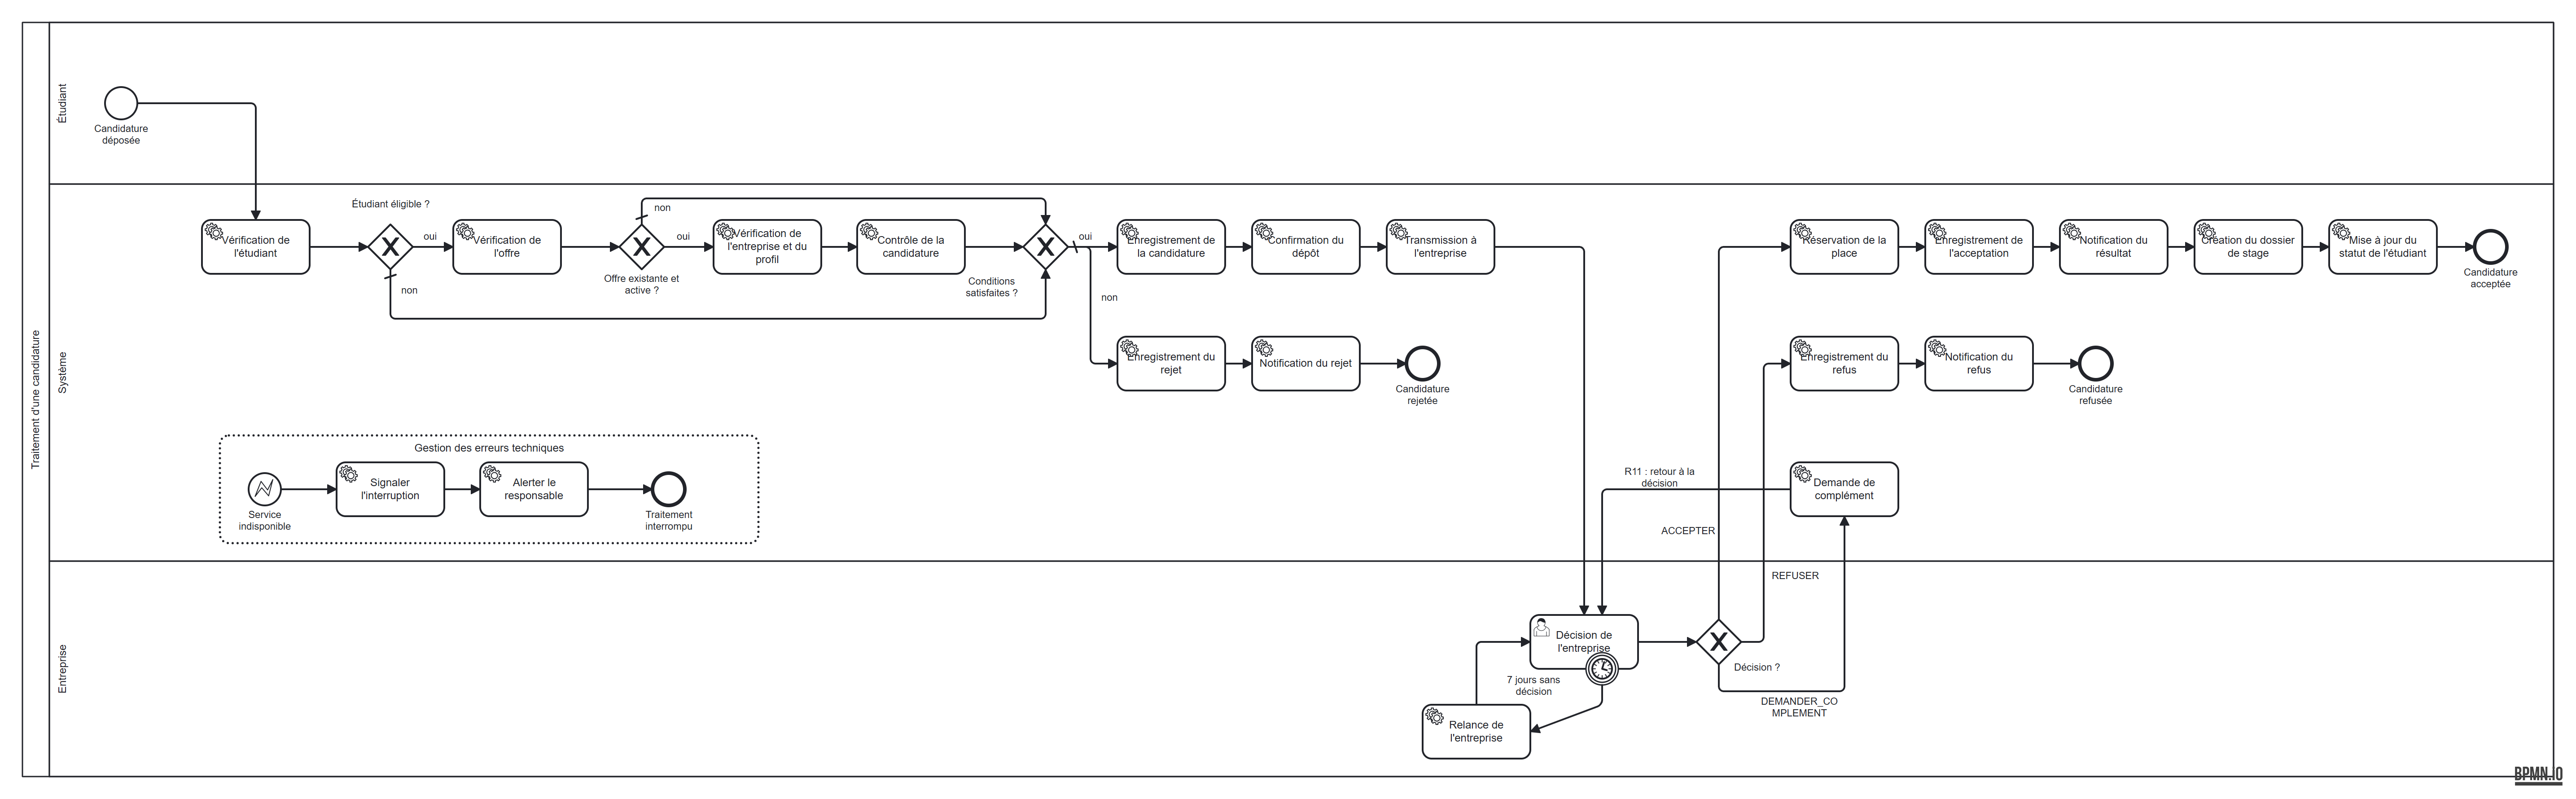
\includegraphics[width=\linewidth]{bpmn-processus.png}
\caption{Processus « Candidature » : diagramme BPMN (rendu par bpmn-js depuis \code{processus-candidature.bpmn})}\label{fig:bpmn-export}
\end{sidewaysfigure}

Le processus existe sous deux formes, qui partagent les mêmes tâches, passerelles et noms :
\begin{itemize}
  \item \textbf{le modèle} (figure~\ref{fig:bpmn-export}) : fichier BPMN à importer dans Bonita Studio, avec des connecteurs SOAP et REST et le sous-processus d'erreur ; sa construction est décrite pas à pas dans \code{docs/bonita/GUIDE\_BONITA.md} ;
  \item \textbf{la version déployée} : construite par programme avec l'API du moteur Bonita (\code{docs/bonita/deploiement}), empaquetée en archive \code{bpmn/Candidature--1.0.bar} et déployée par l'API REST de Bonita (\code{scripts\textbackslash deployer-bonita.ps1}). Elle utilise le \emph{mode secours} du guide : chaque tâche de service est une opération Groovy qui appelle elle-même les services, sans connecteur. Les connecteurs SOAP et REST ne sont en effet pas fournis avec Bonita Community 2025.2 ; ils s'ajoutent depuis la Marketplace.
\end{itemize}
C'est la version déployée qui a été vérifiée de bout en bout face au vrai Bonita (section~\ref{sec:bpmn-verification}).

\begin{figure}[H]
\centering
{\setlength{\fboxsep}{0pt}\color{filet}\fbox{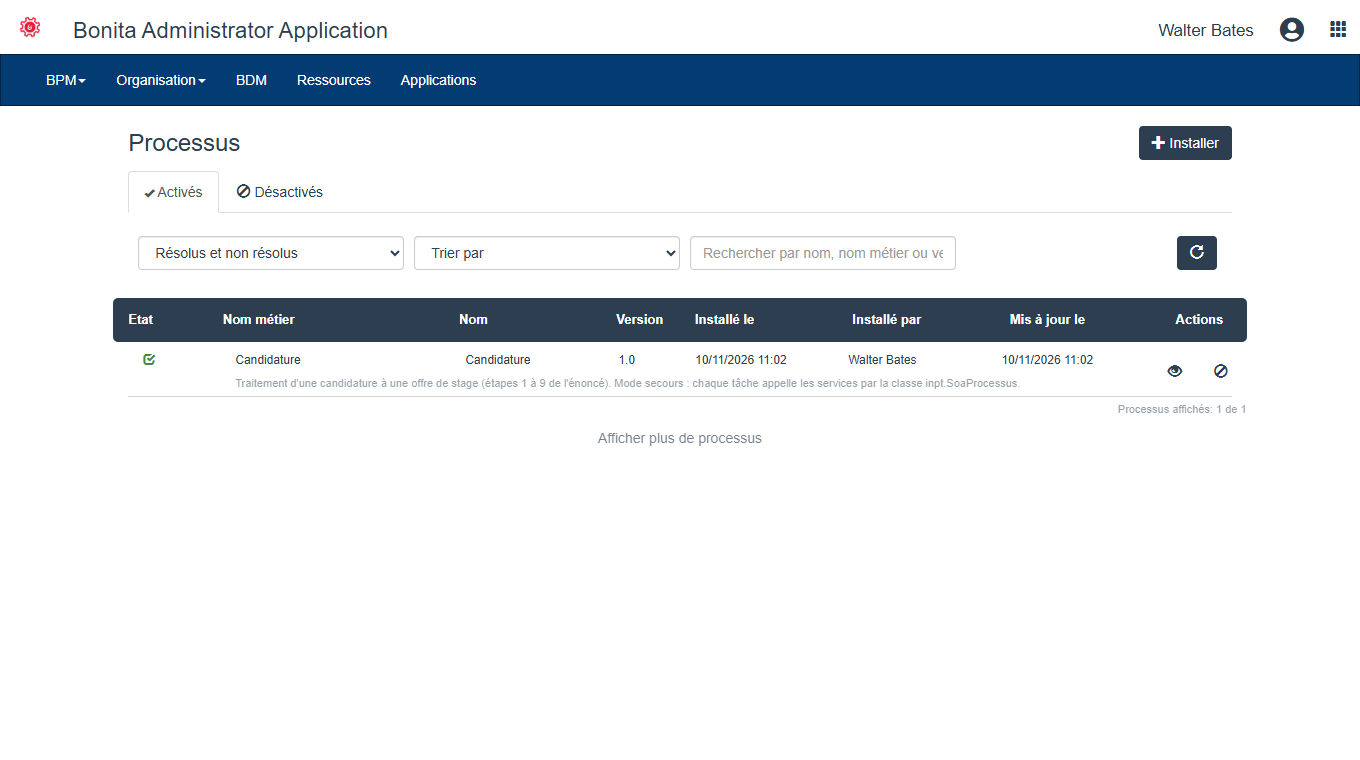
\includegraphics[width=0.9\linewidth]{bonita-processus.png}}}
\caption{Le processus « Candidature » 1.0 déployé et activé dans Bonita (application d'administration)}\label{fig:bonita-processus}
\end{figure}

\section{Déclenchement et données du processus}

S4 démarre un cas par l'API REST de Bonita : connexion (\code{/loginservice}, jeton \code{X-Bonita-API-Token}), recherche du processus par nom et version, puis instanciation avec le contrat suivant.

\begin{table}[H]
\centering\small
\begin{tabularx}{\linewidth}{@{}l l>{\raggedright\arraybackslash}X@{}}
\toprule
\textbf{Entrée du contrat} & \textbf{Type} & \textbf{Rôle} \\ \midrule
\code{soumissionId} & LONG & Soumission créée par S4 ; permet au processus d'écrire dans le bon dossier (journal, rejet, enregistrement). \\
\code{etudiantId} & LONG & Étudiant qui candidate. \\
\code{offreId} & LONG & Offre visée. \\
\code{lettreMotivation} & TEXT & Lettre transmise à l'entreprise. \\
\bottomrule
\end{tabularx}
\caption{Contrat d'instanciation du processus}\label{tab:contrat-bonita}
\end{table}

Le processus n'a qu'une variable, \code{dossier} (une table associative), initialisée à partir du contrat et complétée par chaque tâche (résultat des vérifications, règle violée, identifiant de la candidature, décision…). Avec une seule variable, chaque tâche n'a qu'une opération, et la logique d'appel et de lecture des réponses est regroupée dans une classe Groovy, \code{inpt.SoaProcessus}, livrée dans l'archive du processus et testée hors de Bonita.

\section{Étapes du processus}

\begin{longtable}{@{}>{\raggedright\arraybackslash}p{0.05\linewidth}>{\raggedright\arraybackslash}p{0.27\linewidth}>{\raggedright\arraybackslash}p{0.40\linewidth}>{\raggedright\arraybackslash}p{0.20\linewidth}@{}}
\caption{Tâches du processus et services appelés}\label{tab:taches-bpmn}\\
\toprule \textbf{Étape} & \textbf{Élément BPMN} & \textbf{Appels} & \textbf{Règles} \\ \midrule
\endfirsthead
\toprule \textbf{Étape} & \textbf{Élément BPMN} & \textbf{Appels} & \textbf{Règles} \\ \midrule
\endhead
\bottomrule
\endlastfoot
1 & Candidature déposée (début) & déclenché par S4 à la réception & – \\
2 & Vérification de l'étudiant & SOAP S1 \code{verifierEtudiant} & R1 \\
3 & Vérification de l'offre & SOAP S3 \code{verifierDisponibilite} & R2 (offre) \\
3 & Vérification de l'entreprise et du profil & SOAP S3 \code{consulterOffre}, S2 \code{verifierEntreprise}, S3 \code{verifierCompatibilite} & R2 (entreprise), R7 \\
4 & Contrôle de la candidature & REST S4 \code{verification-doublon}, compte des actives ; date et places d'après S3 & R3 à R6 \\
5 & Passerelle « Conditions satisfaites ? » & – & – \\
5 & Enregistrement de la candidature & REST S4 \code{POST /candidatures} & R5, R6 (garanties) \\
5 & Enregistrement du rejet, Notification du rejet & REST S4 \code{POST /soumissions/\{id\}/rejet}, S5 notification & – \\
6 & Confirmation du dépôt, Transmission à l'entreprise & REST S5 (deux notifications) & – \\
7 & Décision de l'entreprise (tâche humaine) & contrat \{\code{decision}, \code{commentaire}\} & R9 \\
8 & Notification du résultat / du refus & REST S5 & – \\
9 & Réservation de la place & SOAP S3 \code{decrementerPlaces} & R10 \\
9 & Enregistrement de l'acceptation / du refus & REST S4 \code{PATCH /candidatures/\{id\}/statut} & R9 \\
9 & Création du dossier de stage & REST S6 \code{POST /stages} & R10 \\
9 & Mise à jour du statut de l'étudiant & SOAP S1 \code{changerStatutEtudiant} & R10 \\
– & Demande de complément & REST S5, puis retour à la décision & R11 \\
– & Relance de l'entreprise (minuteur de 7 jours) & REST S5 & – \\
\end{longtable}

Chaque tâche inscrit son étape dans le journal de S4 (\code{POST /soumissions/\{id\}/etapes}) : le portail suit ainsi le cas Bonita en direct.

\section{Passerelles de décision}

Les conditions sont des expressions Groovy sur la variable \code{dossier}. Chaque passerelle a un flux par défaut, emprunté si aucune condition n'est vraie : le processus ne peut jamais rester bloqué sur une passerelle.

\begin{table}[H]
\centering\small
\begin{tabularx}{\linewidth}{@{}l l>{\raggedright\arraybackslash}X@{}}
\toprule
\textbf{Passerelle} & \textbf{Flux} & \textbf{Condition} \\ \midrule
Étudiant éligible ? & oui & \code{dossier.etudiantEligible == true} \\
 & non (défaut) & vers la passerelle de décision, qui rejettera (R1) \\
Offre existante et active ? & oui & \code{SoaProcessus.offreValable(dossier)} \\
 & non (défaut) & vers la passerelle de décision (R2) \\
Conditions satisfaites ? & oui & \code{SoaProcessus.conditionsSatisfaites(dossier)} \\
 & non (défaut) & enregistrement du rejet, notification, fin « Candidature rejetée » \\
Décision ? & ACCEPTER & \code{SoaProcessus.decisionEst(dossier, 'ACCEPTER')} \\
 & REFUSER & \code{SoaProcessus.decisionEst(dossier, 'REFUSER')} \\
 & DEMANDER\_COMPLEMENT & \code{SoaProcessus.decisionEst(dossier, 'DEMANDER\_COMPLEMENT')} \\
\bottomrule
\end{tabularx}
\caption{Conditions des passerelles}\label{tab:passerelles}
\end{table}

Les deux passerelles intermédiaires (« Étudiant éligible ? », « Offre existante et active ? ») ne figurent pas dans l'énoncé. Sans elles, un étudiant ou une offre inexistants feraient échouer l'appel suivant (une offre inconnue n'a pas d'entreprise à vérifier) et le cas partirait en erreur technique, alors qu'il s'agit d'un rejet métier ordinaire. Elles court-circuitent les vérifications devenues inutiles et mènent directement à la passerelle de décision de l'étape~5, qui reste le seul point de rejet.

\section{Tâche humaine et boucle de complément}

« Décision de l'entreprise » est une tâche humaine du couloir Entreprise. Son contrat attend une \code{decision} (ACCEPTER, REFUSER ou DEMANDER\_COMPLEMENT, contrainte vérifiée par Bonita) et un \code{commentaire}. L'entreprise décide depuis le portail du projet : S4 vérifie d'abord la règle R10 (une place est-elle encore disponible ?), puis recherche la tâche du cas, se l'assigne et l'exécute par l'API de Bonita.

La demande de complément (R11) passe par la tâche « Demande de complément », qui notifie l'étudiant, puis revient à la décision. Un minuteur de sept jours, en bordure de la tâche humaine, déclenche « Relance de l'entreprise » si aucune décision n'est prise ; la tâche de décision est ensuite recréée. La figure~\ref{fig:bonita-tache} montre un cas en attente : la tâche humaine et son minuteur sont actifs.

\begin{figure}[H]
\centering
{\setlength{\fboxsep}{0pt}\color{filet}\fbox{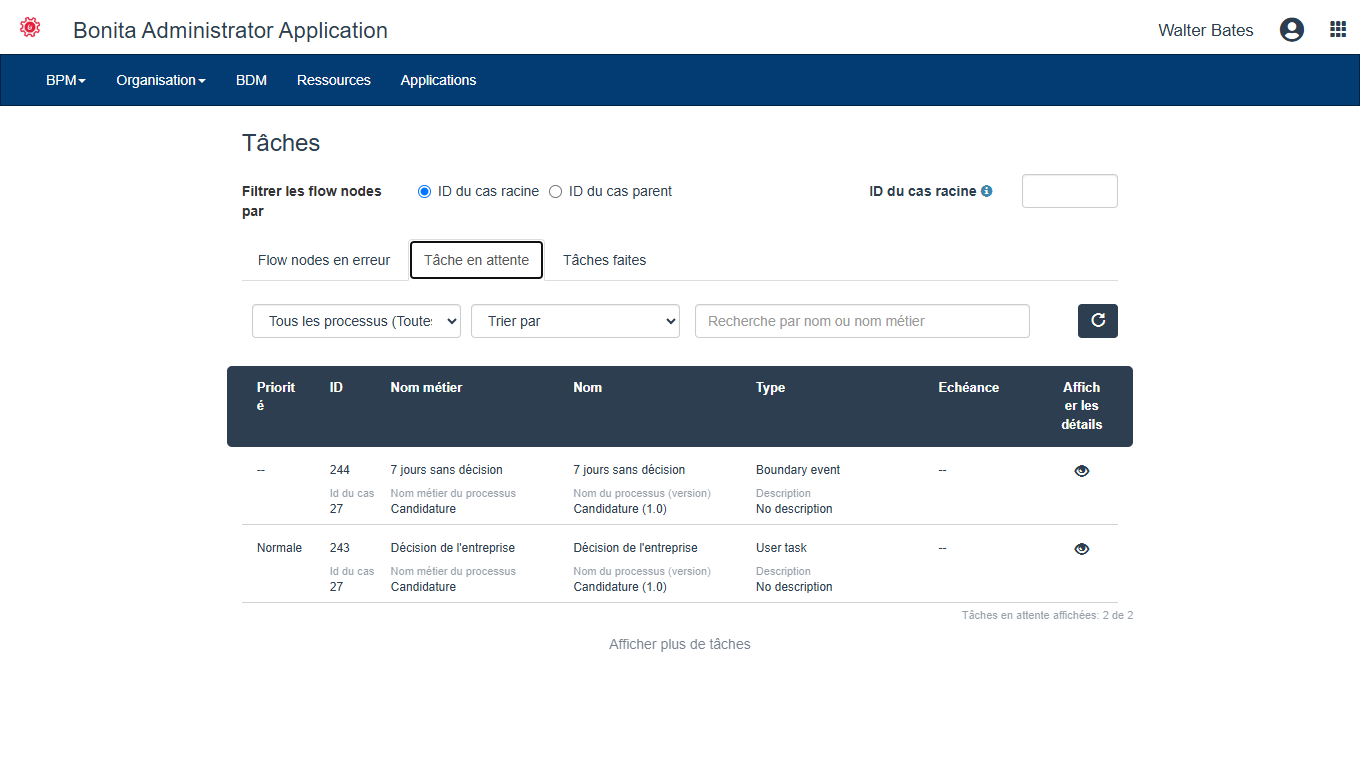
\includegraphics[width=0.9\linewidth]{bonita-tache-decision.png}}}
\caption{Dans Bonita : la tâche « Décision de l'entreprise » en attente, avec son minuteur de relance}\label{fig:bonita-tache}
\end{figure}

\section{Gestion des erreurs et des indisponibilités}

\subsection{Dans le modèle}
Chaque connecteur est configuré pour lever l'erreur BPMN \code{SERVICE\_INDISPONIBLE} s'il échoue (délai dépassé, réponse 5xx, faute \code{ServiceIndisponibleFault}). Un unique sous-processus événementiel, « Gestion des erreurs techniques », intercepte cette erreur où qu'elle survienne : « Signaler l'interruption » (S4 passe la soumission en \statut{ERREUR}, avec la dernière étape réussie), « Alerter le responsable » (courriel \code{ALERTE\_RESPONSABLE}), puis fin « Traitement interrompu ». Un seul sous-processus plutôt qu'un événement de bordure par tâche garde le diagramme lisible et garantit un traitement identique quelle que soit l'étape interrompue.

\subsection{Dans la version déployée}
Sans connecteur, une panne ne peut pas lever d'erreur BPMN : c'est la classe Groovy qui fait le même traitement. Quand un service ne répond pas, la méthode de la tâche signale l'interruption à S4 (soumission en \statut{ERREUR}), envoie l'alerte au responsable, puis échoue : la tâche apparaît « en erreur » dans Bonita (figure~\ref{fig:bonita-erreur}), où un administrateur peut la rejouer une fois le service rétabli. Côté portail, l'étudiant voit « Traitement interrompu » ; aucune candidature à moitié enregistrée ne subsiste.

\begin{figure}[H]
\centering
{\setlength{\fboxsep}{0pt}\color{filet}\fbox{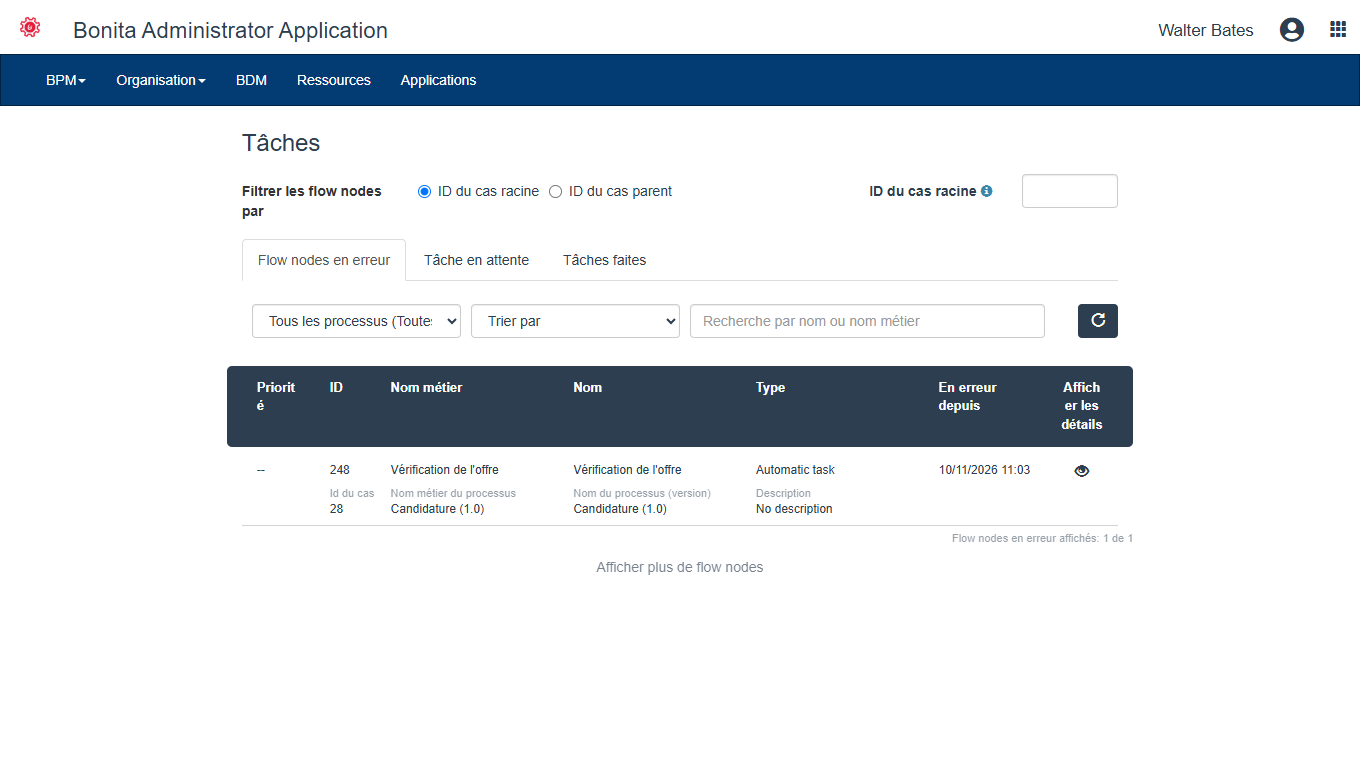
\includegraphics[width=0.9\linewidth]{bonita-taches.png}}}
\caption{Dans Bonita : la tâche « Vérification de l'offre » en erreur pendant une panne de S3}\label{fig:bonita-erreur}
\end{figure}

\section{Connecteurs du modèle}

\subsection{Connecteurs SOAP}
Dans le modèle, les tâches qui appellent S1, S2 ou S3 utilisent le connecteur Web Service (SOAP~1.1) de Bonita. L'enveloppe est produite par la classe Groovy (par exemple \code{SoaProcessus.enveloppeVerifierEtudiant(dossier)}) et contient l'en-tête WS-Security du compte \code{bonita} ainsi que l'identifiant de corrélation du cas. La sortie \code{responseDocumentBody} est lue par la méthode \code{apres…} correspondante, qui met à jour \code{dossier} et inscrit l'étape dans le journal de S4.

\subsection{Connecteurs REST}
Les tâches qui appellent S4, S5 ou S6 utilisent le connecteur REST, avec les en-têtes \code{X-API-Key} (clé du client \code{bonita}), \code{X-Correlation-Id} et \code{Content-Type: application/json}. Les URL et les corps sont, eux aussi, fournis par la classe Groovy. Pour les deux changements de statut (\code{PATCH}), un connecteur qui ne propose pas ce verbe peut envoyer \code{POST} avec l'en-tête \code{X-HTTP-Method-Override: PATCH}, accepté par les services.

\subsection{Mode secours}
En mode secours, la version déployée, chaque tâche est réduite à une seule opération Groovy qui fait l'appel elle-même (par exemple \code{SoaProcessus.verifierEtudiant(dossier)}), avec les mêmes enveloppes SOAP, en-têtes de sécurité et corrélation que les connecteurs. Le comportement métier est identique.

\section{Exécution et vérification}\label{sec:bpmn-verification}

Le processus est vérifié à trois niveaux :
\begin{itemize}
  \item le fichier BPMN est relu sans avertissement par bpmn-moddle, l'analyseur de bpmn-js ;
  \item une simulation (\code{tests/bonita/SimulationBonita.groovy}) répond à l'API REST de Bonita et déroule le graphe tâche par tâche avec la classe livrée, avec connecteurs comme en mode secours ;
  \item surtout, le test de bout en bout a été joué face au \textbf{vrai Bonita Community 2025.2}, processus déployé : les 59 vérifications des scénarios et les 6 de la panne de S3 ont réussi, chaque candidature passant par un cas Bonita.
\end{itemize}

\begin{figure}[H]
\centering
{\setlength{\fboxsep}{0pt}\color{filet}\fbox{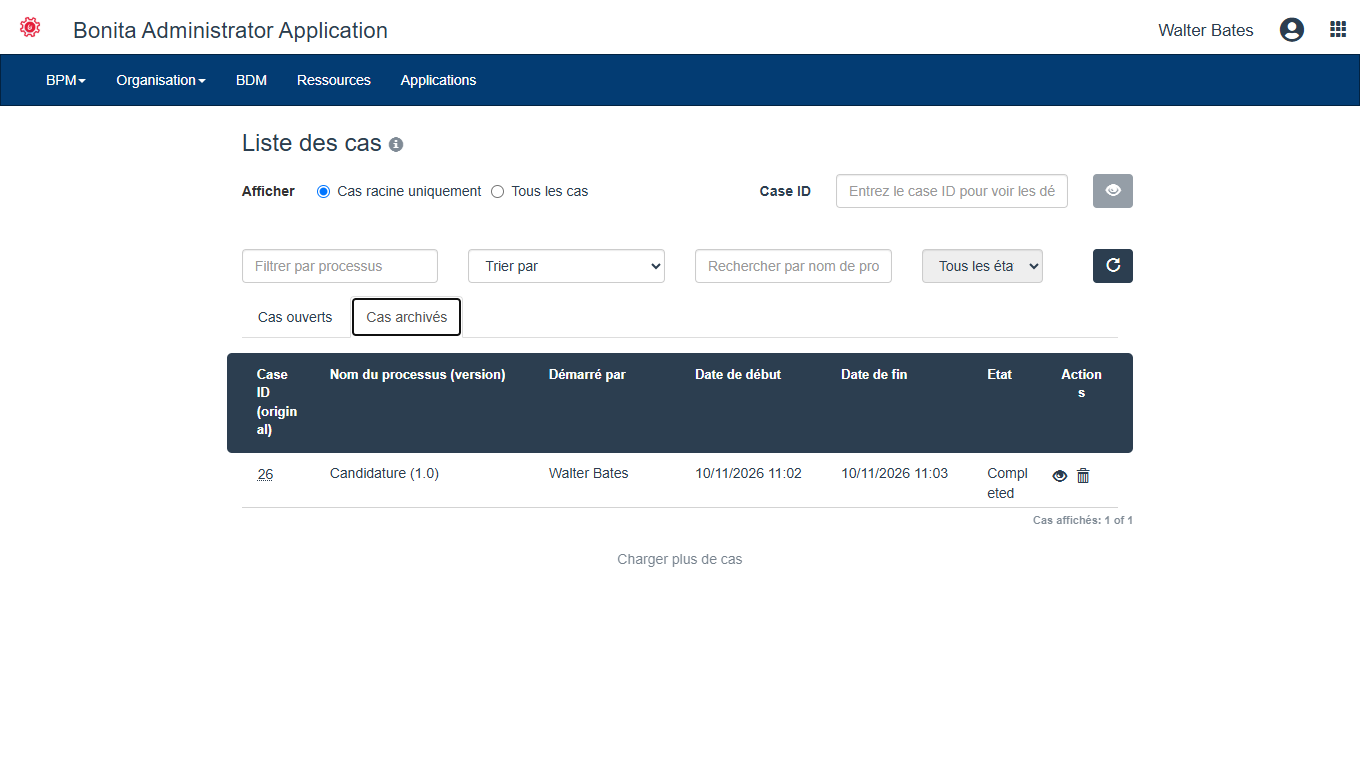
\includegraphics[width=0.9\linewidth]{bonita-cas-archives.png}}}
\caption{Dans Bonita : le cas d'une candidature acceptée, terminé et archivé}\label{fig:bonita-termine}
\end{figure}

Les captures Bonita de ce chapitre sont produites par \code{scripts\textbackslash captures-bonita.ps1}, qui redéploie le processus, joue trois cas réels (acceptation, attente de décision, panne de S3) et capture l'application d'administration de Bonita.

\chapter{Sécurité et gestion des erreurs}\label{chap:securite}

\section{Sécurité des échanges SOAP}\label{sec:securite-soap}

Chaque appel à S1, S2 ou S3 doit porter un en-tête WS-Security \emph{UsernameToken} avec un mot de passe de type \emph{PasswordText} (listing~\ref{lst:wsse}). Un gestionnaire JAX-WS commun (\code{GestionnaireSecuriteServeur}) le vérifie avant que la requête n'atteigne le service ; seule la lecture du WSDL reste publique.

\begin{lstlisting}[language=XMLfr, caption={En-tête WS-Security attendu (compte du processus Bonita)}, label={lst:wsse}]
<wsse:Security xmlns:wsse="http://docs.oasis-open.org/wss/2004/01/oasis-200401-wss-wssecurity-secext-1.0.xsd">
  <wsse:UsernameToken>
    <wsse:Username>bonita</wsse:Username>
    <wsse:Password>Bonita#Ws2026</wsse:Password>
  </wsse:UsernameToken>
</wsse:Security>
\end{lstlisting}

Quatre comptes de service existent, un par client : \code{portail}, \code{bonita}, \code{services} (appels entre services) et \code{soapui} (tests). Le serveur ne connaît que leurs hachages BCrypt, lus dans la configuration (variable d'environnement \code{SOA\_WS\_COMPTES} en production) ; chaque appel accepté est journalisé avec le nom du compte, ce qui permet de savoir qui a fait quoi.

\begin{table}[H]
\centering\small
\begin{tabularx}{\linewidth}{@{}>{\raggedright\arraybackslash}X l@{}}
\toprule
\textbf{Situation} & \textbf{\code{faultcode}} \\ \midrule
En-tête de sécurité absent & \code{wsse:InvalidSecurity} \\
\code{Username} ou \code{Password} manquant & \code{wsse:InvalidSecurity} \\
Mot de passe de type \emph{digest} & \code{wsse:UnsupportedSecurityToken} \\
Compte inconnu ou mot de passe faux & \code{wsse:FailedAuthentication} \\
\bottomrule
\end{tabularx}
\caption{Refus d'authentification SOAP}\label{tab:wsse}
\end{table}

Le mot de passe en clair dans l'en-tête n'est acceptable que sur un canal chiffré : c'est l'objet de la section~\ref{sec:tls}.

\section{Sécurité des API REST}

Chaque client des services REST possède sa clé, transmise dans l'en-tête \code{X-API-Key} : portail, processus Bonita, appels entre services et tests Postman. Les services ne stockent que l'empreinte SHA-256 des clés. Une clé absente ou inconnue donne 401. Certaines opérations sont en outre réservées à certains clients : seul le processus (ou le mode direct) peut enregistrer une candidature ou un rejet, par exemple ; un autre client reçoit 403. Retirer l'accès d'un client revient à supprimer sa clé de la configuration, sans toucher aux autres.

\section{Sécurité du portail}

\begin{itemize}
  \item \textbf{Mots de passe} hachés par BCrypt ; la comparaison prend le même temps qu'un compte existe ou non.
  \item \textbf{Sessions} : un jeton aléatoire de 256 bits est remis à la connexion et envoyé ensuite dans \code{Authorization: Bearer}. La base n'en garde que l'empreinte SHA-256 ; la session expire au bout de huit heures et la déconnexion la supprime.
  \item \textbf{Rôles} vérifiés côté serveur pour chaque ressource (\statut{ETUDIANT}, \statut{ENTREPRISE}, \statut{RESPONSABLE}) : 401 sans session valide, 403 hors de son espace. Une ressource qui appartient à un autre utilisateur (la candidature d'un autre étudiant, le dossier d'une autre entreprise) répond 404, pour ne pas révéler son existence.
  \item \textbf{Masquage} : quand une entreprise consulte un candidat, le portail masque son courriel et son téléphone (\code{s***@inpt.ac.ma}, \code{06******12}) avant l'envoi. Le test de bout en bout vérifie que le JSON reçu par l'entreprise ne contient aucune coordonnée complète.
  \item \textbf{Interface} : tout texte venant des données est inséré comme texte (\code{textContent}), jamais comme HTML ; les courriels affichés dans l'interface le sont dans un cadre isolé (\code{iframe sandbox}) sans aucun droit.
\end{itemize}

\section{Données et configuration}

\begin{itemize}
  \item \textbf{Moindre privilège en base} : chaque service a son compte MySQL, limité à la lecture et à l'écriture des données de son schéma. Un test de socle vérifie qu'un service ne peut ni lire le schéma d'un autre, ni modifier la structure du sien.
  \item \textbf{Requêtes paramétrées} partout (\code{PreparedStatement}) : aucune concaténation de données dans le SQL.
  \item \textbf{Aucun secret dans le code} : adresses, mots de passe, hachages et clés sont dans la configuration et se remplacent par variables d'environnement. Les valeurs du dépôt sont des valeurs de démonstration.
  \item \textbf{Aucune donnée réelle} : personnes, entreprises et numéros sont fictifs, et les courriels restent dans Mailpit.
\end{itemize}

\section{Activer TLS en production}\label{sec:tls}

La démonstration fonctionne en HTTP sur une seule machine, sur l'interface locale uniquement (127.0.0.1) : des certificats auto-signés auraient perturbé SoapUI, Postman, Bonita et le navigateur sans rien protéger de plus sur un poste isolé. En production, nous recommandons :
\begin{enumerate}
  \item un \textbf{reverse proxy} (Nginx ou un API gateway) devant le portail, avec un certificat d'une autorité reconnue, TLS~1.2 minimum et l'en-tête HSTS ; le portail ne serait plus joignable directement ;
  \item \textbf{TLS entre services}, avec une autorité de certification interne, et de préférence l'authentification mutuelle (mTLS), qui authentifie aussi le service appelant ;
  \item conserver WS-Security et les clés d'API par-dessus TLS : TLS protège le transport, les jetons identifient le client applicatif ;
  \item placer les secrets dans un coffre (variables d'environnement injectées au déploiement) et les renouveler régulièrement.
\end{enumerate}
Côté code, seules les adresses changent (\code{https://…}) : elles sont toutes dans la configuration.

\section{Gestion des erreurs}

\subsection{Principes}
\begin{itemize}
  \item \textbf{Erreurs prévues, réponses prévues} : faute SOAP typée ou corps JSON uniforme, avec un code stable et un message en français. Aucune trace technique n'est renvoyée au client ; elle est écrite dans le journal du service avec l'identifiant de corrélation.
  \item \textbf{Validation à l'entrée} : tout champ invalide est signalé, avec la liste complète des problèmes (pas seulement le premier).
  \item \textbf{Codes justes} : 400 pour une requête illisible, 422 pour des données invalides, 409 pour une règle de gestion, 503 pour une indisponibilité, 500 seulement pour l'inattendu.
\end{itemize}

\subsection{Indisponibilité d'un service}
Une panne est traitée à chaque niveau.

\begin{table}[H]
\centering\small
\begin{tabularx}{\linewidth}{@{}l>{\raggedright\arraybackslash}X@{}}
\toprule
\textbf{Niveau} & \textbf{Comportement} \\ \midrule
Appel sortant & Délais de connexion (2~s) et de lecture (5 à 8~s) ; l'échec devient une erreur « service indisponible » nommant le service (\code{SERVICE\_OFFRES\_INDISPONIBLE}). \\
Base de données & Pool de connexions avec délai de 3~s ; l'échec devient 503 (REST) ou \code{ServiceIndisponibleFault} (SOAP) ; \code{GET /health} répond 503. \\
Processus BPMN & Sous-processus d'erreur : soumission en \statut{ERREUR}, responsable alerté par courriel (chapitre~\ref{chap:bpmn}). \\
Mode direct & Même comportement : S4 marque la soumission en \statut{ERREUR}, alerte le responsable et répond 503. \\
Après une acceptation & Si S6 ou S1 ne répondent pas, l'étape échoue mais la décision est conservée ; le responsable relance le suivi une fois le service rétabli (création du stage idempotente). \\
Portail & Les pages qui composent plusieurs services restent affichées : si S3 est arrêté, la liste des candidatures s'affiche avec « détails momentanément indisponibles » au lieu d'échouer. Le tableau de bord du responsable indique l'état des six services. \\
\bottomrule
\end{tabularx}
\caption{Traitement d'une indisponibilité}\label{tab:pannes}
\end{table}

Ces comportements sont vérifiés par de vraies pannes : la suite SoapUI arrête S3, S1 puis MySQL et contrôle les fautes renvoyées ; le test de bout en bout arrête S3 pendant un dépôt et vérifie la soumission en erreur, la réponse 503, l'alerte reçue par le responsable et l'état affiché par le portail (chapitre~\ref{chap:tests}).

\subsection{Traçabilité}
Chaque ligne de journal porte l'identifiant de corrélation de la requête (listing~\ref{lst:trace}). Les historiques métier complètent les journaux techniques : historique des statuts d'une candidature (date, acteur, commentaire), journal des étapes du processus, historique des opérations d'un stage, et historique d'envoi de chaque courriel avec son éventuelle erreur SMTP.

\chapter{Scénarios de test et résultats}\label{chap:tests}

\section{Stratégie}

Les tests sont organisés en quatre niveaux, du plus rapide au plus complet. Chacun se lance par un script et produit un rapport ; les chiffres de ce chapitre sont lus dans ces rapports par \code{rapport/outils/resultats\_tests.py}, qui refuse de produire un tableau si une source manque ou contient un échec.

\begin{table}[H]
\centering\small
\begin{tabularx}{\linewidth}{@{}l>{\raggedright\arraybackslash}X l@{}}
\toprule
\textbf{Niveau} & \textbf{Ce qui est vérifié} & \textbf{Commande} \\ \midrule
Unitaire et composant & Règles et services sans base (DAO en mémoire), échanges SOAP et REST sur serveur embarqué, conformité aux contrats. & \code{build.ps1} \\
Intégration & DAO sur la vraie base MySQL : contraintes, index R5, verrou R6, retrait de place R10. & \code{build.ps1 clean verify} \\
Service & Chaque opération SOAP (SoapUI) et REST (Postman), y compris sécurité, erreurs et vraies pannes. & \code{tests-soapui.ps1}, \code{tests-postman.ps1} \\
Bout en bout & Tous les scénarios joués par le portail, courriels vérifiés dans Mailpit, panne de S3, interface dans un navigateur. & \code{test-bout-en-bout.ps1}, \code{captures-ui.ps1} \\
\bottomrule
\end{tabularx}
\caption{Niveaux de test}\label{tab:niveaux-tests}
\end{table}

Les tests de service et de bout en bout modifient les données : ils sont joués sur une base fraîche (\code{reset-db.ps1}). Les données de démonstration fournissent un étudiant différent pour chaque scénario, pour que l'ordre des scénarios n'influe pas sur leur résultat.

\section{Scénarios fonctionnels}

Le tableau~\ref{tab:scenarios} présente les scénarios principaux, leur résultat attendu et le résultat obtenu lors de la dernière exécution du test de bout en bout (orchestration \modeBoutEnBout{}, processus simulé). La colonne « Obtenu » indique le nombre de vérifications du test qui couvrent le scénario ; toutes ont réussi.

\begin{longtable}{@{}>{\raggedright\arraybackslash}p{0.30\linewidth}>{\raggedright\arraybackslash}p{0.44\linewidth}>{\raggedright\arraybackslash}p{0.20\linewidth}@{}}
\caption{Scénarios, résultats attendus et obtenus}\label{tab:scenarios}\\
\toprule \textbf{Scénario} & \textbf{Attendu} & \textbf{Obtenu} \\ \midrule
\endfirsthead
\toprule \textbf{Scénario} & \textbf{Attendu} & \textbf{Obtenu} \\ \midrule
\endhead
\bottomrule
\endlastfoot
\lignes{generes/tests-scenarios.tex}
\end{longtable}

Le même test passe à l'identique en mode direct, en mode bonita face au processus simulé avec connecteurs, et en mode bonita sans connecteur (mode secours) : \nbBoutEnBout{} vérifications à chaque fois, panne de S3 comprise. Chaque scénario vérifie aussi le courriel reçu dans Mailpit (destinataire, sujet, motif du rejet).

\section{Tests JUnit}

\begin{table}[H]
\centering\small
\begin{tabularx}{\linewidth}{@{}X r r r@{}}
\toprule
\textbf{Module} & \textbf{Unitaires} & \textbf{Sur MySQL} & \textbf{Échecs} \\ \midrule
\lignes{generes/tests-junit.tex}
\bottomrule
\end{tabularx}
\caption{Résultats JUnit par module (\nbJunit{} tests)}\label{tab:junit}
\end{table}

Au-delà des règles de gestion, ces tests couvrent la validation des entrées, les transitions de statut, la sécurité (jetons WS-Security, clés d'API, sessions et rôles du portail), le masquage, le format des erreurs, la propagation de la corrélation et la conformité des routes REST aux contrats OpenAPI. Les tests du mode bonita utilisent un faux serveur Bonita qui répond à l'API REST, pour vérifier l'instanciation, l'exécution de la tâche de décision et la reprise de session.

\section{Tests SoapUI}

Le projet SoapUI (\code{tests/soapui/Stages-SOA-soapui-project.xml}) contient six suites. Les trois premières testent chaque opération des trois services : cas nominaux, conformité de la réponse au WSDL, fautes attendues, données invalides, sécurité (sans en-tête, compte inconnu, mauvais mot de passe). Les trois suivantes provoquent de vraies pannes : le script arrête S3, puis S1, puis la base MySQL, vérifie les fautes \code{ServiceIndisponibleFault} et les réponses dégradées, puis redémarre ce qu'il a arrêté.

\begin{table}[H]
\centering\small
\begin{tabularx}{\linewidth}{@{}X r r r@{}}
\toprule
\textbf{Suite} & \textbf{Cas de test} & \textbf{Assertions} & \textbf{Échecs} \\ \midrule
\lignes{generes/tests-soapui.tex}
\bottomrule
\end{tabularx}
\caption{Résultats SoapUI (\nbSoapUI{} assertions)}\label{tab:soapui}
\end{table}

% TODO capture : SoapUI, projet ouvert, suite « S1 Étudiants » exécutée (cas de test au vert).
\capture{soapui-suite-s1.png}{60mm}{SoapUI : suite « S1 Étudiants » exécutée}{fig:soapui-suite}
% TODO capture : SoapUI, requête verifierEtudiant avec l'en-tête WS-Security et la réponse.
\capture{soapui-requete.png}{60mm}{SoapUI : requête \code{verifierEtudiant} avec en-tête WS-Security}{fig:soapui-requete}

\section{Tests Postman et Newman}

La collection Postman (\code{tests/postman/Stages-SOA.postman\_collection.json}, avec l'environnement \code{Stages-SOA-local}) compte dix dossiers joués dans l'ordre : sécurité des API, parcours nominal, un rejet par règle R1 à R7, R5 et R6 à l'enregistrement, R8 et R9, R10 (dernière place), R11, validation et erreurs de S4, notifications, suivi des stages. Elle est exécutée en ligne de commande par Newman, qui produit un rapport HTML.

\begin{encadre}[Résultat de la dernière exécution]
\nbPostmanRequetes{} requêtes, \nbPostman{} assertions, 0 échec.
\end{encadre}

% TODO capture : Postman, collection « Stages SOA - services REST » et résultat du Runner (toutes les assertions au vert).
\capture{postman-runner.png}{60mm}{Postman : exécution de la collection}{fig:postman-runner}
% TODO capture : rapport HTML de Newman (tests/postman/rapports/rapport-newman.html), page de synthèse.
\capture{newman-rapport.png}{60mm}{Rapport HTML de Newman}{fig:newman}

\section{Interface dans un navigateur}

Le script \code{captures-ui.ps1} pilote Microsoft Edge avec Playwright : il joue une candidature jusqu'à son acceptation par l'interface, visite les vingt-huit écrans des trois espaces et échoue à la moindre erreur dans la console du navigateur, réponse 5xx ou fichier manquant. Les captures du chapitre suivant en sont issues. Ce test a révélé deux défauts corrigés avant la livraison : le message de déconnexion qui disparaissait, et un double affichage à la connexion.

\section{Reproduire les résultats}

\begin{lstlisting}[language={}, caption={Rejouer l'ensemble des tests (PowerShell, à la racine du projet)}]
.\scripts\reset-db.ps1
.\scripts\build.ps1 clean verify            # JUnit, dont tests sur MySQL
.\scripts\start-all.ps1 -Orchestration direct
.\scripts\verifier-socle.ps1                # socle et donnees de demonstration
.\scripts\tests-soapui.ps1                  # SoapUI, pannes comprises
.\scripts\tests-postman.ps1                 # Postman (Newman), base reinitialisee
.\scripts\test-bout-en-bout.ps1             # scenarios par le portail, Mailpit, panne
.\scripts\captures-ui.ps1                   # interface dans Edge
python rapport\outils\resultats_tests.py    # reporte les chiffres dans le rapport
\end{lstlisting}

\chapter{Interface graphique}\label{chap:interface}

\section{Principes}

L'interface, proposée en bonus par l'énoncé, est servie par le portail (\url{http://localhost:8090}). Elle est écrite en HTML, CSS et JavaScript sans framework ni étape de construction : une page unique, des modules JavaScript par espace, un routage par l'adresse (\code{\#/espace/page/identifiant}). Toutes les données passent par l'API du portail, qui applique les rôles et le masquage ; le navigateur n'appelle jamais les services directement.

La charte reste sobre et institutionnelle : le bleu de l'INPT comme seule couleur d'accent, un fond papier, des filets fins, Source Serif~4 pour les titres et Public Sans pour le texte, toutes deux servies par le portail (aucune ressource externe : l'interface fonctionne hors ligne). Les couleurs d'état sont réservées aux statuts et toujours accompagnées d'un libellé en français.

Les captures de ce chapitre ont été produites automatiquement par le parcours Playwright décrit au chapitre précédent, sur les données de démonstration.

\ecran{ui-connexion.png}{860}{860}{0.8}{Connexion, avec les comptes de démonstration}{fig:ui-connexion}

\section{Espace étudiant}

L'étudiant consulte les offres ouvertes (date limite non dépassée, au moins une place), filtrables par texte et par filière. Pour chaque offre, l'interface indique si son profil est compatible (règle R7) et le score indicatif de compétences. Il dépose sa candidature avec une lettre de motivation et obtient aussitôt le résultat du contrôle : enregistrée, ou non recevable avec la règle et le motif.

\ecran{ui-etudiant-offres.png}{860}{1502}{0.8}{Offres de stage et compatibilité avec le profil}{fig:ui-offres}

Le dossier d'une candidature réunit le diagramme du processus, coloré à partir du journal des étapes, la liste des étapes (son équivalent textuel), l'historique des statuts et la lettre. Tant que l'entreprise n'a pas ouvert l'évaluation, l'étudiant peut annuler (R8). Ses courriels sont consultables dans l'espace, tels qu'ils ont été envoyés.

\ecran{ui-etudiant-candidature-acceptee.png}{1000}{2401}{0.8}{Dossier d'une candidature acceptée : processus BPMN en direct et historique}{fig:ui-dossier}

\section{Espace entreprise}

L'entreprise voit les candidatures reçues pour ses offres, avec le profil du candidat et ses coordonnées masquées. Elle ouvre l'évaluation, puis choisit d'accepter, de refuser ou de demander un complément ; un commentaire est obligatoire pour un complément, et toute décision définitive est confirmée dans une boîte de dialogue. Elle gère aussi ses offres (création, modification selon les transitions permises, clôture) et son profil.

\ecran{ui-entreprise-candidature-deposee.png}{1200}{2295}{0.8}{Candidature reçue : profil masqué et ouverture de l'évaluation}{fig:ui-entreprise}

\section{Espace responsable}

Le responsable des stages dispose d'un tableau de bord : offres actives, candidatures et décisions en attente, taux d'acceptation, stages en cours, répartition par statut, état des six services et déclenchement manuel des rappels de date limite. Il consulte toutes les candidatures avec les coordonnées complètes, peut relancer le suivi d'une acceptation interrompue par une panne, gère les étudiants et les entreprises, suit les stages (statut, comptes rendus, évaluations) et recherche dans les courriels envoyés.

\ecran{ui-responsable-tableau-de-bord.png}{1281}{1281}{0.8}{Tableau de bord du responsable des stages}{fig:ui-tableau}

\ecran{ui-responsable-candidature-refusee.png}{900}{2220}{0.8}{Candidature refusée : branche du refus colorée sur le diagramme}{fig:ui-refus}

\section{Vue BPMN en direct}

Le diagramme affiché dans les dossiers est le fichier \code{processus-candidature.bpmn} du processus Bonita, dessiné par la bibliothèque bpmn-js. À l'ouverture d'un dossier, l'interface lit le journal des étapes de la candidature et ajoute un marqueur sur chaque nœud concerné : bleu pour une étape réalisée, rouge pour un rejet ou une erreur, ocre pour l'étape en attente (la décision de l'entreprise). Les flux entre deux étapes réalisées sont également colorés. La branche suivie après la décision (acceptation, refus ou complément) est déduite du détail de l'étape de décision.

Comme les modes direct et bonita écrivent le même journal, la vue est la même quel que soit l'orchestrateur ; en mode bonita, elle suit le cas Bonita au fur et à mesure de son exécution.

\chapter{Déploiement et guide d'exécution}\label{chap:deploiement}

\section{Prérequis}

\begin{table}[H]
\centering\small
\begin{tabularx}{\linewidth}{@{}l l>{\raggedright\arraybackslash}X@{}}
\toprule
\textbf{Outil} & \textbf{Version} & \textbf{Usage} \\ \midrule
JDK & 17 & Compilation et exécution des services (les scripts vérifient la version). \\
Maven & 3.9 & Construction du projet multi-module. \\
Docker Desktop & avec WSL~2 & MySQL 8.4, Mailpit et Adminer. \\
Bonita Studio Community & 2025.2 & Exécution du processus BPMN (mode bonita). \\
SoapUI Open Source & 5.10 & Tests SOAP. \\
Node.js & LTS & Newman, test de bout en bout, Playwright (installés automatiquement par les scripts). \\
Microsoft Edge & – & Parcours de l'interface par Playwright. \\
\bottomrule
\end{tabularx}
\caption{Logiciels nécessaires}\label{tab:prerequis}
\end{table}

Tous les scripts sont en PowerShell et se lancent depuis la racine du projet. Si Windows refuse leur exécution : \code{Set-ExecutionPolicy -Scope CurrentUser RemoteSigned}.

\section{Démarrage}

\begin{lstlisting}[language={}, caption={Démarrage complet}]
.\scripts\start-all.ps1 -Rebuild -Orchestration direct   # construit, demarre Docker puis les 7 services
.\scripts\check-health.ps1                               # etat de chaque service
\end{lstlisting}

\code{start-all.ps1} démarre les conteneurs (MySQL, Mailpit, Adminer), attend que MySQL soit prêt, puis lance chaque service dans son propre processus Java, journal dans \code{logs/}. Il affiche ensuite l'état de chacun (\code{GET /health}) et le mode d'orchestration. Au premier démarrage, MySQL crée les sept schémas, les comptes de service et les données de démonstration (\code{db/init}).

\begin{table}[H]
\centering\small
\begin{tabularx}{\linewidth}{@{}l>{\raggedright\arraybackslash}X@{}}
\toprule
\textbf{Composant} & \textbf{Adresse} \\ \midrule
Interface (portail) & \url{http://localhost:8090} \\
Services SOAP (WSDL) & \url{http://localhost:8081/ws/etudiants?wsdl}, \code{:8082/ws/entreprises?wsdl}, \code{:8083/ws/offres?wsdl} \\
Services REST (Swagger UI) & \url{http://localhost:8084/docs/}, \code{:8085/docs/}, \code{:8086/docs/} \\
Boîte de courriel Mailpit & \url{http://localhost:8025} \\
Administration MySQL (Adminer) & \url{http://localhost:8088} (serveur \code{mysql}) \\
Bonita & \url{http://localhost:8080/bonita} \\
\bottomrule
\end{tabularx}
\caption{Adresses utiles}\label{tab:adresses}
\end{table}

\begin{table}[H]
\centering\small
\begin{tabular}{@{}lll@{}}
\toprule
\textbf{Rôle} & \textbf{Identifiant} & \textbf{Mot de passe} \\ \midrule
Responsable des stages & \code{responsable@inpt.ac.ma} & \code{Responsable@2026} \\
Étudiante & \code{salma.elidrissi@inpt.ac.ma} & \code{Etudiant@2026} \\
Entreprise & \code{contact@novapay-maghreb.ma} & \code{Entreprise@2026} \\
\bottomrule
\end{tabular}
\caption{Comptes de démonstration (tous les étudiants et entreprises ont un compte)}\label{tab:comptes}
\end{table}

\section{Mode d'orchestration}

\begin{itemize}
  \item \textbf{bonita} (par défaut) : le processus doit être déployé dans Bonita. Bonita Studio ouvert (il démarre le serveur Bonita), une commande suffit : \code{.\textbackslash scripts\textbackslash deployer-bonita.ps1}. La version à connecteurs se construit à la main dans le Studio en suivant \code{docs/bonita/GUIDE\_BONITA.md}. S4 vérifie au démarrage que Bonita répond ; sinon, \code{start-all} l'indique et les dépôts répondent 503.
  \item \textbf{direct} : aucune dépendance à Bonita ; S4 exécute les mêmes étapes. C'est le mode des tests automatiques.
\end{itemize}

Le mode se choisit au démarrage : \code{start-all.ps1 -Orchestration bonita} ou \code{direct}.

\section{Configuration}

Chaque paramètre a une valeur par défaut adaptée à la démonstration et peut être remplacé, sans recompiler, par une variable d'environnement (nom en majuscules, points remplacés par des soulignés : \code{soa.db.port} devient \code{SOA\_DB\_PORT}).

\begin{table}[H]
\centering\small
\begin{tabularx}{\linewidth}{@{}l>{\raggedright\arraybackslash}X@{}}
\toprule
\textbf{Variable} & \textbf{Rôle} \\ \midrule
\code{ORCHESTRATION\_MODE} & \code{bonita} ou \code{direct} \\
\code{SOA\_DB\_HOTE}, \code{SOA\_DB\_PORT}, \code{SOA\_DB\_PASSWORD} & Base de données \\
\code{SOA\_WS\_URL\_*}, \code{SOA\_REST\_URL\_*} & Adresse de chaque service appelé \\
\code{SOA\_WS\_COMPTES}, \code{SOA\_API\_CLES} & Hachages des comptes WS-Security et des clés d'API acceptés \\
\code{SOA\_WS\_DELAI\_LECTURE\_MS}, \code{SOA\_REST\_DELAI\_LECTURE\_MS} & Délais d'attente des appels \\
\code{BONITA\_URL}, \code{BONITA\_UTILISATEUR}, \code{BONITA\_MOTDEPASSE} & Accès à l'API de Bonita \\
\bottomrule
\end{tabularx}
\caption{Principales variables de configuration}\label{tab:configuration}
\end{table}

\section{Opérations courantes}

\begin{lstlisting}[language={}, caption={Scripts d'exploitation}]
.\scripts\stop-all.ps1          # arrete les services et Docker (donnees conservees)
.\scripts\reset-db.ps1          # remet les bases et Mailpit a l'etat initial
.\scripts\verifier-socle.ps1    # 68 verifications : bases, droits, donnees de demonstration
.\scripts\build.ps1             # compile et lance les tests unitaires
.\rapport\compiler.ps1          # compile ce rapport (XeLaTeX)
\end{lstlisting}

Avant une démonstration, \code{reset-db.ps1} remet les données dans leur état initial : chaque scénario dispose alors de son étudiant (\code{docs/SCENARIOS\_DEMO.md}).

\section{Dépannage}

\begin{table}[H]
\centering\small
\begin{tabularx}{\linewidth}{@{}>{\raggedright\arraybackslash}p{0.34\linewidth}>{\raggedright\arraybackslash}X@{}}
\toprule
\textbf{Symptôme} & \textbf{Cause probable et remède} \\ \midrule
\code{start-all} signale Docker absent & Démarrer Docker Desktop, attendre qu'il soit prêt, relancer. \\
Un service reste à 503 sur \code{/health} & Sa base ne répond pas : \code{docker ps}, puis \code{reset-db.ps1} si besoin ; voir \code{logs/<service>.log}. \\
Dépôt de candidature en 503 en mode bonita & Bonita n'est pas démarré ou le processus n'est pas déployé ; ou démarrer en mode direct. \\
Un rejet R1 inattendu pendant la démonstration & Les données ont été modifiées par un test : \code{reset-db.ps1}. \\
Port déjà utilisé & Une ancienne instance tourne : \code{stop-all.ps1 -ServicesSeuls}. \\
\bottomrule
\end{tabularx}
\caption{Problèmes fréquents}\label{tab:depannage}
\end{table}

\chapter{Limites, améliorations et conclusion}\label{chap:conclusion}

\section{Limites connues}

\begin{itemize}
  \item \textbf{Pas de HTTPS en local.} Les mots de passe WS-Security et les clés d'API circulent en clair sur l'interface locale de la machine. C'est un choix assumé pour la démonstration ; la section~\ref{sec:tls} décrit la mise en production.
  \item \textbf{Une seule instance par service}, sans répartition de charge. Les services sont sans état (hors base), ce qui permettrait de les dupliquer, mais rien n'est prévu pour les découvrir automatiquement.
  \item \textbf{Cohérence entre services.} L'acceptation modifie trois services sans transaction distribuée. L'ordre des étapes, l'idempotence de la création du stage et la reprise par le responsable évitent toute incohérence durable, mais la reprise reste manuelle.
  \item \textbf{Bonita.} La version déployée utilise le mode secours (sans connecteur) : une panne y met la tâche en erreur au lieu de déclencher le sous-processus d'erreur du modèle, et le diagramme n'est pas éditable dans le Studio (il est construit par programme ; la version à connecteurs se construit à la main avec le guide). Le compte technique qui exécute les décisions masque, dans Bonita, l'auteur réel de la décision (connu de S4). Supprimer un cas à l'annulation efface son historique dans Bonita (il reste dans S4).
  \item \textbf{Interface.} Pas de version mobile travaillée ; pas de notification en direct (les écrans se mettent à jour à la navigation) ; le compte de connexion d'un étudiant créé par le responsable n'est pas créé automatiquement.
  \item \textbf{Infrastructure.} Seules la base, Mailpit et Adminer sont conteneurisés ; les services Java se lancent par des scripts PowerShell, donc sous Windows.
\end{itemize}

\section{Améliorations possibles}

\begin{table}[H]
\centering\small
\begin{tabularx}{\linewidth}{@{}l>{\raggedright\arraybackslash}X@{}}
\toprule
\textbf{Amélioration} & \textbf{Apport} \\ \midrule
API gateway & Point d'entrée unique devant les services REST (Kong, Spring Cloud Gateway…) : authentification, quotas, journalisation et TLS centralisés ; le portail ne s'occuperait plus que de l'interface. \\
ESB & Médiation entre SOAP et REST, transformation des messages et routage (Apache Camel, WSO2) : les services n'auraient plus à connaître le protocole des autres. \\
Registre de services & Découverte dynamique des adresses (Consul, Eureka) au lieu d'adresses fixes en configuration ; prérequis pour plusieurs instances. \\
Conteneurisation complète & Une image Docker par service et un \code{docker compose up} unique, puis Kubernetes : démarrage identique sur toute machine, redémarrage automatique, mise à l'échelle. \\
Messagerie asynchrone & Notifications publiées dans une file (RabbitMQ, Kafka) : un serveur de courriel lent ou arrêté ne ralentirait plus le traitement d'une candidature. \\
Saga & Compensations automatiques pour l'acceptation (rendre la place si la création du stage échoue définitivement), au lieu de la reprise manuelle. \\
Identité fédérée & OAuth~2 et OpenID Connect (Keycloak) pour les utilisateurs et les clients techniques, avec jetons signés à durée de vie courte. \\
Observabilité & Traces distribuées (OpenTelemetry) prolongeant l'identifiant de corrélation, métriques et tableaux de bord. \\
Intégration continue & Construction, tests et rapport à chaque modification du dépôt. \\
\bottomrule
\end{tabularx}
\caption{Pistes d'amélioration}\label{tab:ameliorations}
\end{table}

\section{Conclusion}

Ce projet met en œuvre, sur un cas métier concret, les principes d'une architecture orientée services : des services autonomes qui possèdent leurs données, exposent un contrat explicite (WSDL ou OpenAPI) et ne communiquent que par ces contrats ; un processus BPMN qui orchestre ces services pour traiter une candidature de bout en bout ; une sécurité adaptée à chaque type d'échange.

Au-delà des fonctionnalités demandées, nous avons cherché à rendre le système vérifiable : chaque règle de gestion porte un identifiant suivi du code jusqu'aux courriels, chaque contrat est confronté au code par des tests, chaque panne est provoquée réellement pour en vérifier le traitement, et une candidature peut être suivie d'un service à l'autre grâce à un identifiant de corrélation. Les \nbJunit{} tests JUnit, les \nbSoapUI{} assertions SoapUI, les \nbPostman{} assertions Postman et le test de bout en bout ont tous réussi lors de la dernière exécution.

Le projet nous a surtout appris que la difficulté d'une architecture orientée services n'est pas d'écrire chaque service, mais de traiter ce qui se passe entre eux : un service qui ne répond pas, deux demandes simultanées, une étape qui réussit à moitié. Les choix les plus utiles (une soumission distincte de la candidature, un journal d'étapes commun aux deux modes d'orchestration, des opérations idempotentes, un sous-processus d'erreur unique) sont nés de ces questions.


\end{document}
